\chapter{Variedades}

\section{Variedades topológicas e diferenciais}

\subsection{Cartas e atlas}

\begin{definition}
Sejam $V$ um conjunto e $d \in \N$. Uma \emph{carta} $d$-dimensional de $V$ é um par $(A,\x)$ em que $A \subseteq V$ é um conjunto e $\x\colon A \to \R^d$ é uma função injetiva tal que $\x(A)$ é um aberto de $\R^d$. O \emph{domínio} de $(A,\x)$ é $A$, o domínio de $\x$, e o \emph{mapa de coordenadas} de $(A,\x)$ é a função $\x$. A \emph{$i$-ésima coordenada} da carta $(A,\x)$ é a função $\x^i := \pi^i \circ \x\colon A \to \R$.
\end{definition}

\begin{definition}
Sejam $V$ um conjunto e $(A,\x),(\bar A,\bar\x)$ cartas $d$-dimensionais de $V$. A \emph{transição de coordenadas} de $(A,\x)$ para $(\bar A,\bar\x)$ é a função
	\begin{equation*}
	\bar\x \circ \x\inv: \x(A \cap \bar A) \to \bar\x(A \cap \bar A).
	\end{equation*}
\end{definition}

A composição $\bar\x \circ \x\inv$ não está necessariamente definida em todo $\x(A)$, mas somente na interseção do domínio de $\x\inv$ com a imagem inversa do domínio de $\bar\x$ por $\x\inv$. Para ver que esse é o conjunto acima, basta notar que da injetividade de $\x$ segue
	\begin{equation*}
	\x(A) \cap (\x\inv)\inv(\bar A) = \x(A \cap \bar A).
	\end{equation*}
Da mesma forma definimos o contradomínio como acima.

\begin{definition}
Seja $V$ um conjunto. Cartas $\Cont^k$-\emph{compatíveis} de $V$ são cartas $(A,\x)$ e $(\bar A,\bar\x)$ tais que $\x(A \cap \bar A)$ e $\bar\x(A \cap \bar A)$ são abertos e a transição de coordenadas
	\begin{equation*}
	\bar\x \circ \x\inv: \x(A \cap \bar A) \to \bar\x(A \cap \bar A)
	\end{equation*}
é um difeomorfismo $\Cont^k$. Para $k=0$, as cartas são \emph{topologicamente compatíveis}, para $k>0$, são \emph{diferencialmente compatíveis}, sendo para $k=\infty$ \emph{suavemente compatíveis}.
\end{definition}

A relação de compatibilidade entre cartas não é uma relação de equivalência, mas a compatibilidade de atlas, uma noção associada a ela, é. A seguir, definimos o que é um atlas. A primeira condição, além de aparentemente necessária para que todos os pontos de $V$ tenham cartas, será uma hipótese essencial para que a compatibilidade de atlas seja uma relação de equivalência. Isso é um resultado muito simples, mas que indica que nossa axiomatização é boa, de certa forma, pois ao termos a estrutura de um atlas do conjunto, não temos simplesmente várias cartas, mas cartas que se comportam de acordo com certa relação de equivalência. Essa relação de equivalência nos permitirá definir um objeto abstrato chamado atlas maximal, que na prática nunca é calculado, mas que como objeto teórico é belo e conveniente.

\begin{definition}
Seja $V$ um conjunto. Um \emph{atlas} $\Cont^k$ $d$-dimensional de $V$ é um conjunto $\atlas$ de cartas $d$-dimensionais de $V$ tal que
	\begin{enumerate}
	\item (Cobertura) O conjunto $V$ é coberto pelos domínios das cartas de $\atlas$
	\begin{equation*}
	V = \displaystyle\bigcup_{(A,\x) \in \atlas} A;
	\end{equation*}
	\item (Compatibilidade) Todas cartas $(A,\x), (\bar A,\x) \in \atlas$  são $\Cont^k$-compatíveis.
	\end{enumerate}
Para $k=0$, $\atlas$ é um atlas \emph{topológico}, para $k>0$, um atlas \emph{diferencial}, sendo para $k=\infty$ um atlas \emph{suave}.
\end{definition}

Na definição de atlas, se não especificássemos que todas cartas devem ser $d$-dimensionais, poderíamos ter partes do conjunto $V$ que fossem mapeadas em espaços reais de dimensão diferente. No entanto, nas cartas $(A,\x), (\bar A,\bar \x) \in \atlas$ em que $A \cap \bar A \neq \emptyset$, teríamos ao menos um homeomorfismo entre os conjuntos $\x(A \cap \bar A)$ e $\bar\x(A \cap \bar A)$, de modo que as cartas poderiam ser restritas a espaços reais de mesma dimensão; se $k \geq 1$, diferenciando a transição de coordenadas $\bar\x \circ \x\inv$ teríamos um homeomorfismo linear entre os espaços reais, garantindo a mesma dimensão. Isso mostra que, a menos de cartas que não tenham interseção no domínio, teríamos que ter espaços reais de mesma dimensão modelando o conjunto $V$. A partir de agora, sempre consideraremos que os atlas têm a mesma dimensão, e a dimensão de um atlas só será mencionada quando necessário.

\begin{definition}
Seja $V$ um conjunto. Atlas \emph{$\Cont^k$-compatíveis} de $V$ são atlas $\Cont^k$ $\atlas$ e $\bar\atlas$ de $V$ tais que todas as cartas $(A,\x) \in \atlas$ e $(\bar A,\bar\x) \in \bar \atlas$ são $\Cont^k$-compatíveis.
\end{definition}

Essa definição é equivalente a dizer que $\atlas \cup \bar \atlas$ é um atlas $\Cont^k$.

\begin{proposition}
Seja $V$ um conjunto. A relação de $\Cont^k$-compatibilidade de atlas de $V$ é uma relação de equivalência.
\end{proposition}
\begin{proof}
A reflexividade e a simetria são evidentes, pois valem entre cartas. Para conferir a transitividade, sejam $\atlas,\bar\atlas$ e $\{(A_i,\x_i)\}_{i \in I}$ atlas de $V$ e sejam $(A,\x) \in \atlas$ e $(\bar A,\bar\x) \in \bar\atlas$ cartas.
Como $\atlas$ e $\bar\atlas$ são compatíveis com $\{(A_i,\x_i)\}_{i \in I}$, segue que para todo $i \in I$, $\x(A \cap A_i)$ e $\x_i(A_i \cap \bar A)$ são abertos de $\R^d$ e as transições de coordenadas
	\begin{equation*}
	\x_i \circ \x\inv: \x(A \cap A_i) \to \x_i(A \cap A_i).
	\end{equation*}
e
	\begin{equation*}
	\bar\x \circ \x_i\inv: \x_i(A_i \cap \bar A) \to \bar\x(A_i \cap \bar A).
	\end{equation*}
são difeomorfismos $\Cont^k$. Compondo essas transições de coordenada, e notando que
	\begin{equation*}
	\x(A \cap A_i) \cap (\x_i \circ \x\inv)\inv(\x_i(A_i \cap \bar A)) = \x(A \cap A_i \cap \bar A)
	\end{equation*}
(e analogamente para $\bar\x(A \cap A_i \cap \bar A)$), concluímos que
	\begin{equation*}
	(\bar\x \circ \x_i\inv) \circ (\x_i \circ \x\inv): \x(A \cap A_i \cap \bar A) \to \bar\x(A \cap A_i \cap \bar A)
	\end{equation*}
e é um difeomorfismo $\Cont^k$.

Agora, notemos que o conjunto $\x(A \cap A_i \cap \bar A)$ é um aberto de $\R^d$ já que $\x(A \cap A_i)$ e $\x_i(A_i \cap \bar A)$ são abertos e $\x_i \circ \x\inv$ é contínua. Como
	\begin{equation*}
	V= \bigcup_{i \in I} A_i,
	\end{equation*}
segue que
	\begin{equation*}
	\bigcup_{i \in I} \x(A \cap A_i \cap \bar A) = \x\left(A \cap \bigcup_{i \in I} A_i \cap \bar A\right) = \x(A \cap \bar A),
	\end{equation*}
então $\x(A \cap \bar A)$ é aberto de $\R^d$. Analogamente, o contradomínio de $\bar\x \circ \x\inv$ é $\bar\x(A \cap \bar A)$ e é aberto de $\R^d$. Portanto $\bar\x \circ \x\inv$ é uma função bem definida em $\x(A \cap \bar A)$ e segue que
	\begin{equation*}
	\bar\x \circ \x\inv: \x(A \cap \bar A) \to \bar\x(A \cap \bar A).
	\end{equation*}
é um difeomorfismo $\Cont^k$, o que mostra que $(A,\x)$ e $(\bar A,\bar\x)$ são $\Cont^k$-compatíveis, e finalmente $\atlas$ e $\bar\atlas$ são $\Cont^k$-compatíveis.
\end{proof}

Isso implica, em particular, que os atlas $\Cont^k$ $d$-dimensionais de $V$ podem ser particionados em classes de equivalência. Além disso, segue da proposição anterior que se dois atlas são compatíveis, sua união é um atlas, o que motiva a próxima definição.

\begin{definition}
Seja $V$ um conjunto. Um atlas \emph{maximal} $\Cont^k$ (ou uma \emph{estrutura diferencial $\Cont^k$}) $d$-dimensional de $V$ é a união de todos os atlas de uma classe de equivalência de atlas $\Cont^k$ $d$-dimensionais de $V$.
\end{definition}

Como comentado acima, o atlas maximal é um atlas, pois é uma união de atlas compatíveis. Com essa definição, podemos finalmente definir uma variedade.

\subsection{Variedades e estrutura topológica e diferencial}

\begin{definition}
Uma \emph{variedade} $\Cont^k$ $d$-dimensional é um par $\bm V=(V,\atlas)$ em que $V$ é um conjunto e $\atlas$ é um atlas maximal $\Cont^k$ $d$-dimensional de $V$. Para $k=0$, a variedade $\bm V$ é uma variedade \emph{topológica} e, para $k>0$, é uma variedade \emph{diferencial}, sendo para $k=\infty$ uma variedade \emph{suave}.
\end{definition}

Quando não for necessário explicitar detalhes, uma variedade $\Cont^k$ $d$-dimensional será simplesmente referida como uma variedade. Denotamos ainda a dimensão da variedade por um expoente: $\bm V^d$. É possível mostrar que toda variedade diferencial tem um subatlas maximal suave, de modo que não há perda de informação quando se separam as variedades apenas em topológicas e diferenciais, mas isso não será feito aqui.

%\begin{definition}
%Seja $\bm V$ uma variedade. Para $p \in V$, uma \emph{carta} em $p$ é uma carta $(A,\x) \in \atlas$ tal que $p \in A$, e a \emph{$i$-ésima coordenada} com respeito a $(A,\x)$ é a função
%	\begin{align*}
%	\func{\x_i}{A}{\R}{p}{\pi_i \circ \x(p)}
%	\end{align*}
%\end{definition}

\begin{definition}
Seja $\bm V$ uma variedade. A \emph{topologia} de $\bm V$ é o conjunto
	\begin{equation*}
	\topo \coloneqq  \ger{\bigcup_{(A,\x) \in \atlas} \x\pux(\topo_{\R^d})},
	\end{equation*}
em que $\topo_{\R^d}$ é a topologia de $\R^d$.
\end{definition}

Na notação acima, $\ger{C}$ denota a topologia gerada pelo conjunto $C \subseteq \p(V)$ e $\x\pux(\topo)$ denota a topologia puxada de $\topo$ pela função $\x$, ou seja, o conjunto de imagens inversas por $\x$ de abertos da topologia $\topo$. Essa é a menor topologia tal que todos os mapas de coordenadas $\x$ das cartas do atlas maximal são contínuos, a topologia inicial com respeito aos mapas de coordenadas do atlas da variedade. Pode-se ver que essa é a topologia cuja base são os domínios das cartas do atlas maximal. Ainda, vale notar que essa é a mesma topologia da gerada pelas topologias puxadas de $\topo|_{\x(A)}$, a topologia induzida de $\topo$ em $\x(A)$. Isso ocorre porque os mapas de coordenadas $\x$ são bijeções no seu domínio, logo puxam qualquer subconjunto de $\x(A)^\complement$ no vazio. De fato, há várias definições equivalentes de como induzir uma topologia em uma variedade, e a acima parece ser a mais bem definida em questão de teoria; no entanto, em geral só conseguimos conhecer um atlas de uma variedade, e não o atlas maximal todo, portanto saber gerar a topologia sem precisar do atlas maximal seria uma ferramenta muito boa, essencial às vezes. É isso que as proposições a seguir oferecem. A primeira afirma que, se gerarmos uma topologia a partir de uma atlas, qualquer carta compatível com esse atlas terá um mapa de coordenadas contínuo, o que implica, em particular, que as topologias geradas pelo atlas maximal e as geradas por qualquer subatlas são a mesma.

\begin{proposition}
Sejam $V$ um conjunto, $\atlas=\{(A_i,\x_i)\}_{i \in I}$ um atlas de $V$ e
	\begin{equation*}
	\topo := \ger{\bigcup_{i \in I} {\x_i}\pux(\topo_{\R^d})}.
	\end{equation*}
Se $(A,\x)$ é uma carta compatível com $\atlas$, então $\x$ é uma função contínua.
\end{proposition}
\begin{proof}
Seja $U$ um aberto de $\R^d$. Para todo $i \in I$, definamos $U_i := (\x \circ \x_i\inv)(\x_i(A_i))$ e $S := \R^d \setminus \bigcup_{i \in I} U_i$. Então
	\begin{equation*}
	U = U \cap \R^d = \bigcup_{i \in I} (U \cap U_i) \cup (U \cap S).
	\end{equation*}
Como $V=\bigcup_{i \in I} A_i$ e, para todo $i \in I$, $\x\inv(U_i) = A \cap A_i$, então
	\begin{align*}
	\x\inv(S) &= \x\inv(\R^d) \cap \x\inv\left(\left(\bigcup_{i \in I} U_i\right)^\complement\right) \\
		&= A \cap \left(\bigcup_{i \in I} \x\inv(U_i) \right)^\complement \\
		&= A \cap \left(\bigcup_{i \in I} A \cap A_i \right)^\complement \\
		&= A \cap (A \cap V)^\complement = A \cap (A)^\complement = \emptyset.
	\end{align*}
Disso, segue que $\x\inv(U \cap S)=\emptyset$ e, portanto,
	\begin{align*}
	\x\inv(U) &= \bigcup_{i \in I} \x\inv(U \cap U_i) \cup \x\inv(U \cap S) \\
		&= \bigcup_{i \in I} (A \cap A_i) \cup (A \cap\emptyset) \\
		&= \bigcup_{i \in I} A \cap A_i.
	\end{align*}
Mostraremos, agora, que $A \cap A_i$ é aberto para todo $i \in I$, e com isso concluiremos que $\x\inv$ é aberto. Para isso, notemos que
	\begin{equation*}
	\x_i(A \cap A_i) = \x_i(A_i) \cap (\x_i \circ \x\inv)(\x(A)).
	\end{equation*}
Como $\x(A)$ é aberto, pois $(A,\x)$ é carta, e $\x \circ \x_i\inv$ é difeomorfismo, pois $(A,\x)$ é compatível com $\atlas$, então $(\x_i \circ \x\inv)(\x(A))$ é aberto e, portanto, $\x_i(A \cap A_i)$ é aberto, o que implica que $\x_i\inv(\x_i(A \cap A_i)) = A \cap A_i$ é aberto. Assim, concluímos que $\x\inv(U)$ é aberto de $\topo$, portanto $\x$ é contínua.
\end{proof}

\begin{proposition}
Sejam $\bm V=(V,\atlas)$ uma variedade e $\bar\atlas$ um atlas compatível com o atlas maximal $\atlas$. A topologia
	\begin{equation*}
	\bar\topo := \ger{\bigcup_{(A,\x) \in \bar\atlas} \x\pux(\topo_{\R^d})},
	\end{equation*}
é igual à topologia $\topo$ de $\bm V$.
\end{proposition}
\begin{proof}
Por definição da topologia de $\bm V$, temos imediatamente que $\bar\topo \subseteq \topo$. Para a inclusão contrária, a proposição anterior mostra que toda carta de $\atlas$ tem mapa de coordenadas contínuo em $\bar\topo$, o que implica que $\topo \subseteq \bar\topo$.
\end{proof}

Uma consequência óbvia das definições é que qualquer subconjunto aberto de $\R^d$ é uma variedade. Antes de continuar a discussão sobre as propriedades topológicas de variedades, um comentário importante é que alguns autores definem uma variedade a partir de um espaço topológico desde o início, exigindo que os mapas de coordenadas sejam homeomorfismos com sua imagem no espaço real. A partir dessa definição, a topologia da variedade já existe desde o começo e não é induzida pelas cartas.

\begin{exercise}
Sejam $(\bm V_i)_{i \in [n]} = ((V_i,\atlas_i))_{i \in [n]}$ variedades $\Cont^k$ de dimensões $(d_i)_{i \in [n]}$, respectivamente. O par
	\begin{equation*}
	\prod_{i \in [n]} V_i = \left( \prod_{i \in [n]} V_i, \prod_{i \in [n]} \atlas_i \right),
	\end{equation*}
em que $\prod_{i \in [n]} V_i$ é o produto de conjuntos e
	\begin{equation*}
	\prod_{i \in [n]} \atlas_i := \set{ \left(\prod_{i \in [n]} A_i, \prod_{i \in [n]} \x_i \right)}{\forall_{i \in [n]} (A_i,\x_i) \in \atlas_i}
	\end{equation*}
é uma variedade $\Cont^k$ de dimensão $\sum_{i \in [n]} d_i$
% e, para todo $i \in [n]$, as projeções $\proj_i\colon \prod_{i \in [n]} V_i \to V_i$ são $\Cont^k$-diferenciáveis.
\end{exercise}

\begin{comment}
\begin{proof}
Sejam $\left(\prod_{i \in [n]} A_i, \prod_{i \in [n]} \x_i \right),\left(\prod_{i \in [n]} A'_i, \prod_{i \in [n]} \x'_i \right) \in \prod_{i \in [n]} \atlas_i$ cartas. Queremos mostrar que elas são $\Cont^k$-compatíveis. Notemos que
	\begin{equation*}
	\left( \prod_{i \in [n]} A_i \right) \cap \left( \prod_{i \in [n]} A'_i \right) = \prod_{i \in [n]} \left( A_i \cap A'_i \right),
	\end{equation*}
logo
	\begin{align*}
	\left( \prod_{i \in [n]} \x_i \right) \left( \prod_{i \in [n]} A_i \right) \cap \left( \prod_{i \in [n]} A'_i \right) &= \left( \prod_{i \in [n]} \x_i \right) \prod_{i \in [n]} \left( A_i \cap A'_i \right) \\
		&= \prod_{i \in [n]} \x_i\left( A_i \cap A'_i \right),
	\end{align*}
que é aberto pois $\x_i\left( A_i \cap A'_i \right)$ são abertos, já que $(A_i,\x_i)$ e $(A'_i,\x'_i)$ são $\Cont^k$-compatíveis, e
	\begin{equation*}
	\left( \prod \x_i \right) \left( \prod_{i \in [n]} A_i \right) \cap \left( \prod_{i \in [n]} A'_i \right) = \prod_{i \in [n]} \x_i\left( A_i \cap A'_i \right),
	\end{equation*}
que é aberto pois $\x'_i\left( A_i \cap A'_i \right)$ são abertos, já que $(A_i,\x_i)$ e $(A'_i,\x'_i)$ são $\Cont^k$-compatíveis. Agora,
	\begin{align*}
	,
	\end{align*}
\end{proof}

\end{comment}

\subsection{Exemplos de variedades}

\subsubsection{Esfera}

A esfera $d$-dimensional é o conjunto
	\begin{equation*}
	\S^d = \set{x \in \R^{d+1}}{\nor{x}=1}.
	\end{equation*}

A partir dessa notação de esfera unitária, podemos escrever facilmente qualquer $n$-esfera de raio $r \in \R$ e centro $c \in \R^{d+1}$ em $\R^{d+1}$ como $c + r\S^d$ usando a notação de adição e multiplicação de um elemento de um anel com um subconjunto do anel.

Vamos considerar, na esfera, um atlas com apenas duas cartas: as \emph{projeções estereográficas} focadas no norte e no sul.

\begin{definition}
O \emph{polo norte} de $\S^d$ é o ponto $N := \ii_d = (0,\ldots,0,1)$ e a \emph{projeção estereográfica norte} de $\S^d$ é a função
	\begin{align*}
	\func{\pi_N}{\S^d \setminus\{N\}}{\R^d}{x}{\frac{1}{1-x_d}(x_0,\ldots,x_{d-1})}.
	\end{align*}

O \emph{polo sul} de $\S^d$ é o ponto $S := -N = = -\ii_d = (0,\ldots,0,-1)$ e a \emph{projeção estereográfica sul} de $\S^d$ é a função
	\begin{align*}
	\func{\pi_S}{\S^d \setminus\{S\}}{\R^d}{x}{\frac{1}{1+x_d}(x_0,\ldots,x_{d-1})}.
	\end{align*}
\end{definition}

\begin{proposition}
Sejam $\pi_N$ e $\pi_S$ as projeções estereográficas norte e sul de $\S^d$. O conjunto
	\begin{equation*}
	\atlas := \{(\S^d \setminus\{N\},\pi_N),(\S^d \setminus\{S\},\pi_S)\}
	\end{equation*}
é um atlas de $\S^d$.
\end{proposition}
\begin{proof}
As inversas de $\pi_N$ e $\pi_S$ são dadas por
	\begin{align*}
	\func{\pi_N\inv}{\R^d}{\S^d}{x}{\frac{1}{\nor{x}^2 + 1}\left(2x_0,\ldots,2x_{d-1},\nor{x}^2 - 1\right)}
	\end{align*}
e
	\begin{align*}
	\func{\pi_S\inv}{\R^d}{\S^d}{x}{\frac{-1}{\nor{x}^2+1}\left(2x_0,\ldots,2x_{d-1},\nor{x}^2-1\right)}.
	\end{align*}

A transição de coordenadas entre as cartas é dada por
	\begin{align*}
	\func{\pi_N \circ \pi_S\inv}{\R^d \setminus\{0\}}{\R^d \setminus\{0\}}{x}{\frac{1}{\nor{x}^2}x}.
	\end{align*}
Claramente, todas as funções são suaves.
\end{proof}

\begin{figure}
\centering
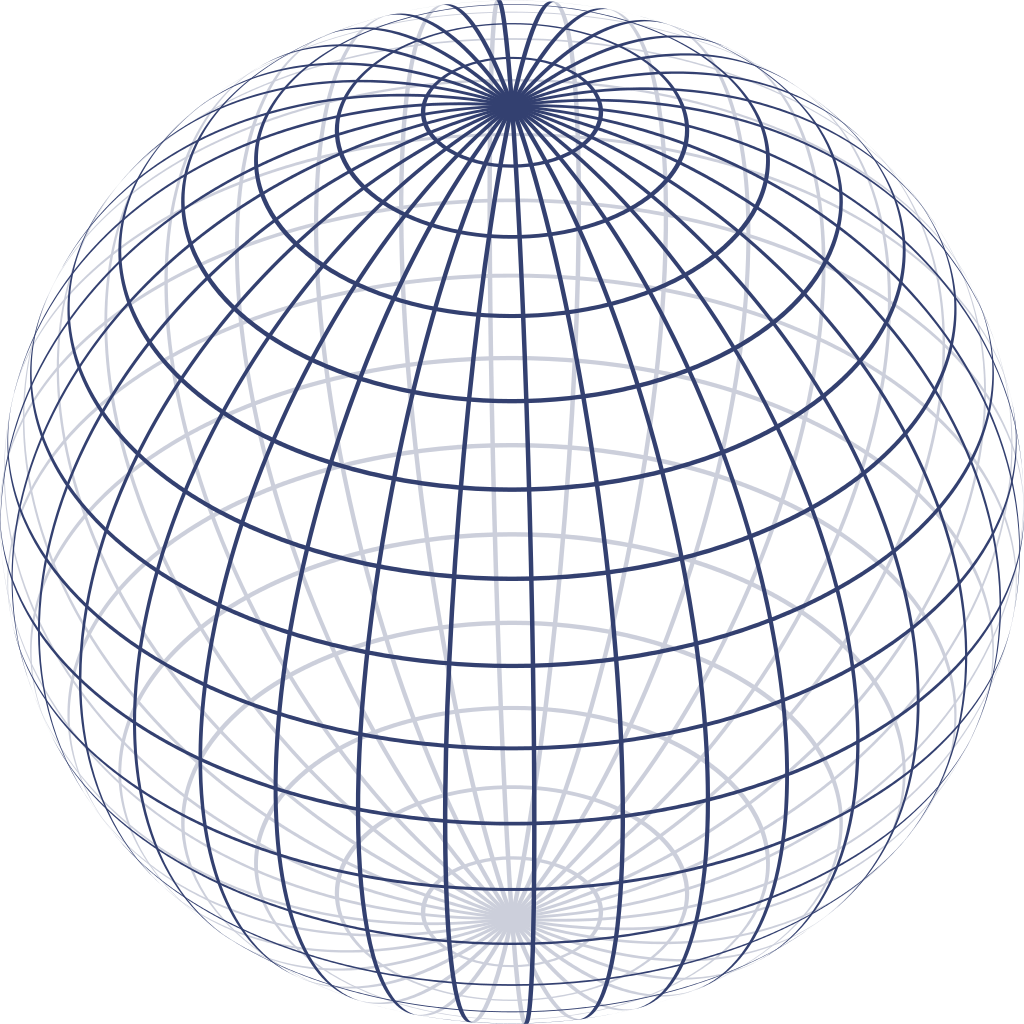
\includegraphics[width=3in]{./imagens/esfera}
\caption{Esfera $2$-dimensional \ensuremath{\S^2}}
\end{figure}

\subsubsection{Espaço projetivo}

\begin{definition}
Sejam $x,y \in \R^d\setminus\{0\}$. A relação de \emph{equivalência homogênea} entre os pontos é definida por
	\begin{equation*}
	x : y \sse \exists t \in \R^* \qquad x = ty.
	\end{equation*}
\end{definition}

Essa relação é realmente uma relação de equivalência, pois tomando $t=1$ temos a reflexividade, tomando $\bar t = t\inv$ temos a simetria e tomando $t_1t_0$ temos a transitividade. A classe de equivalência de um ponto $x \in \R^d$ é a reta sem a origem de $\R^d$ que passa pela origem e por $x$, e é denotada por $[x_0 : \cdots : x_{d-1}] := [x]$.

\begin{definition}
O \emph{espaço projetivo real} $d$-dimensional é o conjunto
	\begin{equation*}
	\pro\R^d := \set{[x_0 : \cdots : x_d]}{x \in \R^{d+1}}.
	\end{equation*}
\end{definition}

Considerando os conjuntos
	\begin{equation*}
	A_i := \set{[x_0 : \cdots : x_d] \in \pro\R^d}{x_i \neq 0}.
	\end{equation*}
e as funções
	\begin{align*}
	\func{\varphi_i}{A_i}{\R^d}{[x_0 : \cdots : x_d]}{\frac{1}{x_i}(x_0,\ldots,x_{i-1},x_{i+1},\ldots,x_d)},
	\end{align*}
cujas inversas são
	\begin{align*}
	\func{\varphi_i\inv}{\R^d}{A_i}{x}{[x_0:\ldots,x_{i-1}:1:x_i:,\ldots:x_{d-1}]}.
	\end{align*}

Uma descrição equivalente é
	\begin{equation*}
	\pro\R^d := \quo{\S^d}{\S^0} = \set{\{x,-x\}}{x \in \S^d}.
	\end{equation*}

Essa construção considera a ação de $\S^0$ em $\S^d$, a saber,
	\begin{align*}
	\func{\times}{\S^0 \times \S^d}{\S^d}{(u,x)}{ux}.
	\end{align*}

O espaço $\S^0 = \{1,-1\} \subseteq \R$ tem estrutura de grupo com a multiplicação de $\R$ e pode ser identificado com o grupo $\Z_2$ pelo isomorfismo de grupos
	\begin{align*}
	\func{h}{(\Z_2,+)}{(\S^0,\times)}{n}{(-1)^n},
	\end{align*}
que é homomorfismo pois $(-1)^{n+n'} = (-1)^n(-1)^{n'}$ e é claramente bijeção.

\subsubsection{Toro}

\begin{definition}
	O \emph{toro} $d$-dimensional é o conjunto
	\begin{equation*}
	\T^d := \R^d / \Z^d.
	\end{equation*}
\end{definition}

\begin{figure}
\centering
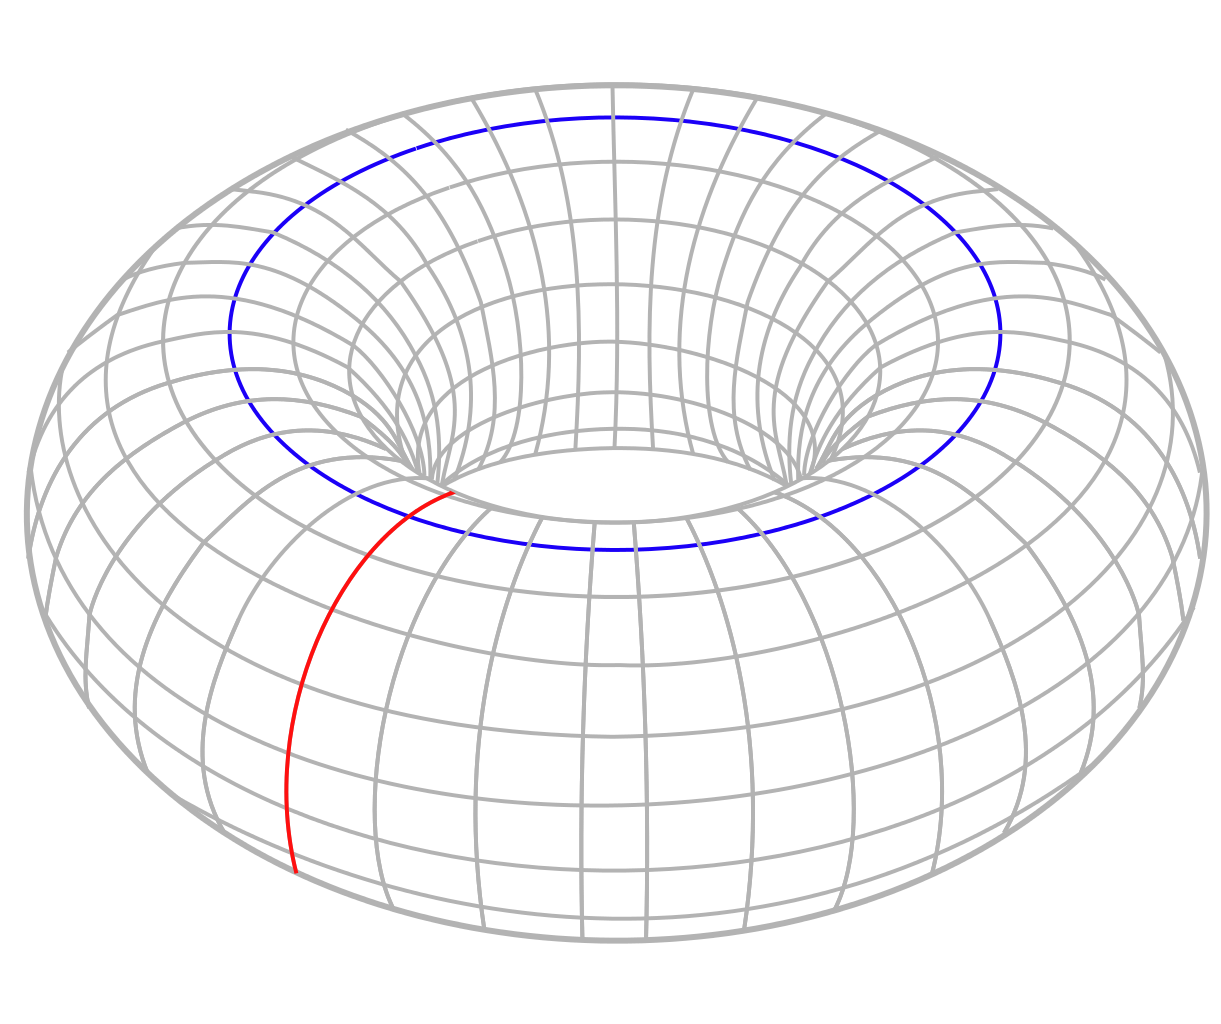
\includegraphics[width=3in]{./imagens/toro}
\caption{Toro}
\end{figure}

\subsubsection{Hiperboloide}

Relembremos que $\R^{1,d}$ é o espaço vetorial $\R^{1+d}$ munido da $2$-forma simétrica não degenerada $\inte{\var}{\var}_{1,d}$ de assinatura $(1,d)$, definida para todos $x,x' \in \R^{1,d}$ por
	\begin{equation*}
	\inte{x}{x'}_{1,d} = x_0x'_0 - \sum_{k=1}^{d} x_k x'_k,
	\end{equation*}
em que $x = (x_0,\ldots,x_d)$ e $x' = (x'_0,\ldots,x'_d)$. A forma quadrática associada a $\inte{\var}{\var}_{1,d}$ é $\qua{\var}_{1,d}$, definida para todo $x \in \R^{1,d}$ por
	\begin{equation*}
	\qua{x}_{1,d} = {x_0}^2 - \sum_{k=1}^{d} {x_k}^2.
	\end{equation*}

\begin{definition}
O \emph{hiperboloide} $d$-dimensional é o conjunto
%	\begin{equation*}
%	\Hip^d := \set{(x,t) \in \R^d \times \R = \R^{d+1}}{\nor{x}^2+1=t^2 \text{\ \ e\ \ } t>0}.
%	\end{equation*}
	\begin{equation*}
	\Hip^d := \set{x \in \R^{1,d}}{\qua{x}_{1,d} = 1 \land x_0 > 0}.
	\end{equation*}
\end{definition}




\subsection{Propriedades topológicas}

Uma variedade definida como acima não precisa necessariamente ser um espaço separado ($T_2$), ou seja, espaço cujos pontos distintos são separados por vizinhanças. Em geral, na definição de variedade consideram-se espaços separados, mas ainda não faremos essa distinção. Ainda, outra hipótese comum é que a topologia admita base enumerável. Isso é equivalente, para uma variedade, a existir um subatlas enumerável.

\begin{proposition}
Seja $\bm V = (V,\atlas)$ uma variedade. Então
	\begin{enumerate}
	\item $\bm V$ é um espaço topológico acessível (T$_1$);

	\item $\bm V$ é um espaço topológico separado (T$_2$) se, e somente se, para todo $p$, $p' \in V$ distintos, existe $(A,\x) \in \atlas$ tal que $p$, $p' \in A$ ou existem cartas $(A,\x)$, $(A',\x) \in \atlas$ tais que $A \cap A' = \emptyset$, $p \in A$ e $p' \in A'$;

	\item $\bm V$ tem base topológica enumerável se, e somente se, existe um subatlas enumerável de $\atlas$;

	\item Cada componente conexa de $\bm V$ é conexa por caminhos.
	\end{enumerate}
\end{proposition}
\begin{proof}
	\begin{enumerate}
	\item Sejam $p,\bar p$ pontos distintos de $V$. Queremos mostrar que existe vizinhança de cada um que não contém o outro. Para isso, tomamos carta $(A,\x)$ em $p$. Se $A$ não contém $\bar p$, então $A$ é vizinhança de $p$ que não contém $\bar p$; caso contrário, como $\x(p)$ e $\x(\bar p)$ são distintos, pois $\x$ é injetiva, segue que existe vizinhança $U$ de $\x(p)$ que não contém $\x(p)$, pois $\R^d$ é acessível, logo $\x\inv(p)$ é uma vizinhança de $p$ que não contém $\bar p$. Analogamente, mostramos o mesmo para $\bar p$, portanto $V$ eles são separados e concluímos que $\bm V$ é um espaço topológico acessível.

	\item Exercício.
%($\Rightarrow$) Suponhamos que $\bm V$ é separado. Para todos $p,p' \in V$ distintos, existem vizinhanças abertas $U$ de $p$ e $U'$ de $p'$ tais que $U \cap U' = \emptyset$.

	\item ($\Rightarrow$) Como $\bm V$ tem base enumerável, então toda cobertura de $V$ tem subcobertura enumerável. Sendo assim, dada a cobertura por abertos das cartas de $\atlas$, tomamos uma subcobertura enumerável e segue que esse é um subatlas enumerável de $\atlas$.

($\Leftarrow$) Seja $\bar \atlas$ um subatlas enumerável de $\atlas$. Para cada $(A,\x) \in \bar \atlas$, consideramos as bolas $\bola{x}{r} \subseteq \x(A) \subseteq \R^d$ tais que $r \in \Q$ e $x \in \Q^d$. A união das imagens inversas dessas bolas pelos mapas de coordenadas é o conjunto enumerável
	\begin{equation*}
	\bar{\mathcal B} = \bigcup_{(A,\x) \in \bar \atlas} \set{\x\inv(\bola{x}{r})}{\bola{x}{r} \subseteq \x(A),  r \in \Q, x \in \Q^d}.
	\end{equation*}
Esse conjunto é uma base de $\bm V$: (1) O conjunto $\bar{\mathcal B}$ cobre $V$, pois os domínios das cartas de $\bar\atlas$ cobrem $V$ e as imagens inversas das bolas de centro e raio racionais cobrem o domínio de cada carta de $\bar\atlas$; (2) Sejam $A_1$ e $A_2 \in \bar{\mathcal B}$. Então $A_1 \cap A_2$ é aberto e, para todo $p \in A_1 \cap A_2$, existem $r \in \Q$ e $x \in \Q^d$ tais que $\x_1(p) \in \bola{x}{r} \subseteq \x_1(A_1 \cap A_2)$, logo $p \in {\x_1}\inv(\bola{x}{r}) \subseteq A_1 \cap A_2$.

	\item Sejam $C(p)$ uma componente conexa de $\bm V$ em $p$ e $U$ o conjunto de todos pontos de $C(p)$ ligados por um caminho a $p$. Mostraremos que $U$ é aberto e fechado, portanto igual a $C(p)$. Mostremos primeiro que $U$ é aberto. Seja $q \in C(p)$ e $A$ uma vizinhança de $q$ homeomorfa a uma bola de $\R^d$. Como a bola é conexa por caminhos e homeomorfa a $A$, segue que $A$ é conexa por caminhos. Portanto todo ponto de $A$ está em $C(p)$, já que existe caminho do um ponto de $A$ a $q$ e caminho de $q$ a $p$. Isso mostra que $U$ é aberto. Agora, seja $q \in U^\complement$. Novamente, tomamos uma vizinhança $A$ de $q$ homeomorfa a uma bola de $\R^d$ e segue que $A$ é conexa por caminhos. Nesse caso, nenhum ponto de $A$ está em $C(p)$, caso contrário existiria caminho ligando $q$ a $p$, o que contradiz a hipótese. Isso mostra que $U^\complement$ é fechado, portanto $U$ aberto. Assim, como $U$ é aberto e fechado, $C(p)$ é conexo e $p \in U$, segue que $C(p)=U$.
		\end{enumerate}
\end{proof}

\section{Funções diferenciáveis}

\subsection{Funções diferenciáveis}

\begin{definition}
Sejam $\bm{V_0}$ e $\bm{V_1}$ $\Cont^k$-variedades de dimensões $d_0$ e $d_1$, respectivamente. Uma função \emph{$\Cont^k$-diferenciável} de $\bm{V_0}$ para $\bm{V_1}$ é uma função
% contínua
 $F\colon V_0 \to V_1$ que satisfaz: para todo $p \in V_0$, existem cartas $(A_0,\x_0) \in \atlas_0$ em $p$ e $(A_1,\x_1) \in \atlas_1$ em $F(p)$ tais que $F(A_0) \subseteq A_1$ e
		\begin{equation*}
		\x_1 \circ F \circ \x_0\inv: \x_0(A_0) \to \x_1(A_1)
		\end{equation*}
é uma função $\Cont^k$-diferenciável de $\x_0(A_0) \subseteq \R^{d_0}$ para $\x_1(A_1) \subseteq \R^{d_1}$. Denota-se $F\colon \bm{V_0} \to \bm{V_1}$. O conjunto das funções $\Cont^k$-diferenciáveis de $\bm{V_0}$ para $\bm{V_1}$ é denotado $\Cont^k(\bm{V_0},\bm{V_1})$. %Quando $V_1=\R$, denota-se simplesmente $\Cont^k(\bm V_0)$.
\end{definition}

A diferenciabilidade independe da carta escolhida no seguinte sentido.

\begin{proof}
Sejam $(A_0,\x_0)$, $(\bar A_0,\bar\x_0)$ cartas em $p$ e $(A_1,\x_1)$, $(\bar A_1,\bar\x_1)$ cartas em $f(p)$ tais que $F(A_0) \subseteq A_1$ e $F(\bar A_0) \subseteq \bar A_1$. Então $F(A_0 \cap \bar A_0) \subseteq A_1 \cap \bar A_1$, $p \in A_0 \cap \bar A_0$ e $F(p) \in A_1 \cap \bar A_1$. Restringindo domínios adequadamente,
	\begin{equation*}
	\bar \x_1 \circ F \circ \bar \x_0\inv = (\bar \x_1 \circ \x_1\inv) \circ (\x_1 \circ F \circ \x_0 \inv) \circ (\x_0 \circ \bar \x_0\inv)
	\end{equation*}
%	\begin{equation*}
%	\coo{F}{\bar \x_0}{\bar \x_1} = \coo{\Id}{\x_1}{\bar \x_1} \circ \coo{F}{\x_0}{\x_1} \circ \coo{\Id}{\bar \x_0}{\x_0}
%	\end{equation*}
Como as transições de coordenadas $(\bar \x_1 \circ \x_1\inv)$ e $(\x_0 \circ \bar \x_0\inv)$ são $\Cont^k$-difeomorfismos, então $(\x_1 \circ F \circ \x_0 \inv)$ é $\Cont^k$-diferenciável se, e somente se, $(\bar \x_1 \circ F \circ \bar \x_0\inv)$ o é.
\end{proof}

Como uma $\Cont^k$-variedade é também uma $\Cont^l$-variedade para todo $l\leq k$, sempre se pode definir entre $\Cont^k$ e $\Cont^l$-variedade funções $\Cont^m$-diferenciáveis para qualquer $m \leq \min\{k,l\}$.

\begin{proposition}
Sejam $\bm{V_0}$ e $\bm{V_1}$ $\Cont^k$-variedades e $F_0: \bm{V_0} \to \bm{V_1}$ uma função $\Cont^k$-diferenciável. Então $F$ é uma função contínua.
\end{proposition}

\begin{proposition}
Sejam $\bm{V_0}$, $\bm{V_1}$ e $\bm{V_2}$ $\Cont^k$-variedades e $F_0: \bm{V_0} \to \bm{V_1}$ e $F_1: \bm{V_1} \to \bm{V_2}$ funções $\Cont^k$-diferenciáveis. Então $F_1 \circ F_0: \bm{V_0} \to \bm{V_1}$ é uma função $\Cont^k$-diferenciável.
\end{proposition}

Casos particulares relevantes são quando uma das duas variedades é um subconjunto de $\R^d$. Toma-se assim a carta trivial nesse subconjunto. Um desses caso é evidenciado a seguir.

\begin{definition}
Sejam $\bm V$ uma $\Cont^k$-variedade e $I \subseteq \R$ um intervalo aberto. Uma \emph{$\Cont^k$-curva} em $\bm V$ é uma função $\gamma: I \to V$ $\Cont^k$-diferenciável.
\end{definition}

Isso é equivalente a dizer que, para todo $p \in \gamma(V)$ existe carta $(A,\x)$ em $p$ tal que
	\begin{equation*}
	\x \circ \gamma: I \to \x(A)
	\end{equation*}
é uma função $\Cont^k$-diferenciável, ao escolher acima a função identidade.

\subsection{Funções separadoras e partições da unidade}

Consideraremos inicialmente a função
	\begin{align*}
	\func{f}{\R}{\R}{x}{\begin{cases}
		0,& x \leq 0 \\
		e^{-\frac{1}{x}},& x > 0.
	\end{cases}}
	\end{align*}
Pode ser mostrado que essa função é suave, mas não faremos isso aqui. Sejam $r_0,r_1 \in \R$ tais que $r_0 < r_1$. Construímos a função
	\begin{align*}
	\func{h}{\R}{\R}{x}{\frac{f(r_1-x)}{f(x-r_0)-f(r_1-x)}}.
	\end{align*}
Essa função é suave e tem a seguinte propriedade: $h(x)=1$ para todo $x \leq r_0$, $0 < h(x) < 1$ para todo $x \in \left ]r_0, r_1\right [$ e $h(x)=0$ para todo $x \geq r_1$. Isso quer dizer que ela é uma função suave que separa (precisamente) os conjuntos $\left ]-\infty,r_0\right ]$ e $\left [r_1,+\infty\right [$. Em $\R^d$, podemos separar (precisamente) por função suave a bola fechada $\bola{0}{r_0}$ e o complementar da bola fechada $\bola{0}{r_1}$. Basta usar a função $h$ para definir a função% $H := h \circ \nor{}$
	\begin{align*}
	\func{H}{\R^d}{\R}{x}{h(\nor{x})}.
	\end{align*}
Uma função suave que separa esses conjuntos é geralmente chamada de uma ``bump function'', mas aqui a chamaremos de função separadora, pois ela separa (precisamente) os conjuntos. Em francês, essa função também é conhecida como uma ``fonction plateau'', algo como ``função planalto''. Essas funções são também chamadas de ``funções teste''.
%Mais geralmente, uma função separadora é uma função que separa (precisamente) seu suporte fechado (onde não é 0) de seu núcleo (fechado) (onde é 0)?
Mais geralmente, uma função como essa é uma função para $[0,1]$ com suporte em um aberto $A$ que vale $1$ em um compacto $K$, ou seja, uma função contínua que separa um fechado $A^\complement$ e um compacto $K$. Essa funções sempre existem em espaços topológicos separados por vizinhanças ($T_2$) e localmente compactos.

\begin{definition}
Sejam $\bm X$ um espaço topológico e $f: X \to \R$ uma função contínua. O \emph{suporte fechado} de $f$ é o conjunto
	\begin{equation*}
	\overline\supp(f) := \overline{\supp(f)}.
	\end{equation*}
\end{definition}

\begin{proposition}
Sejam $\bm X$ um espaço topológico separado por vizinhanças ($T_2$) e localmente compacto, $A \subseteq X$ um aberto e $K \subseteq A$ um compacto. Existe função $f: X \to [0,1]$ tal que $\overline\supp(f) \subseteq A$ e $f(K)=\{1\}$.
\end{proposition}

Notemos que tal função separa continuamente $A^\complement$ e $K$, pois
	\begin{equation*}
	\supp(f) \subseteq \overline\supp(f) \subseteq A
	\end{equation*}
implica $A^\complement \subseteq \supp(f)^\complement$, portanto $f(A^\complement) \subseteq f(\supp(f)^\complement)=\{0\}$.

\begin{definition}
Sejam $\bm X$ um espaço topológico (variedade suave) e $\mathcal C=(C_i)_{i \in I}$ uma cobertura aberta de $\bm X$. Uma \emph{partição da unidade} (\emph{suave}) subordinada a $\mathcal C$ é uma família de funções contínuas (suaves) $\psi_i\colon X \to \R$ tal que
	\begin{enumerate}
	\item (Unidade) Para todos $i \in I$ e $x \in X$, $0 \leq \psi_i(x) \leq 1$;
	\item (Partição) A família $(\overline\supp(\psi_i))_{i \in I}$ é localmente finita (todo ponto tem uma vizinhança que interseciona finitos dos conjuntos da família) e, para todo $x \in X$,
		\begin{equation*}
		\sum_{i \in I} \psi_i(x) = 1.
		\end{equation*}
	\item (Subordinação) Para todo $i \in I$, $\overline\supp(\psi_i) \subseteq C_i$.
	\end{enumerate}
\end{definition}

\begin{proposition}
Sejam $\bm V$ uma variedade (suave) e $\mathcal C = (C_i)_{i \in I}$ uma cobertura aberta de $\bm V$. Existe partição da unidade (suave) $\psi_i\colon X \to \R$ subordinada a $\mathcal C$.
\end{proposition}






\section{Espaço tangente}

A partir desta seção, não estudaremos mais com detalhes os casos de variedades $\Cont^k$-diferenciais para cada $k \in \N \cup \{\infty\}$. Nos referiremos somente a \emph{variedades} ou \emph{variedades diferenciais}, sendo que o primeiro termo se refere a qualquer variedade topológica e o segundo a variedades suaves, isto é, $\Cont^\infty$-diferenciais, e a mesma nomenclatura será usada para funções diferenciáveis.

\subsection{Álgebra dos campos escalares}

Dada uma variedade diferencial $\bm V$, um \emph{campo escalar} em $\bm V$ é uma função do espaço $\Cont^\infty(\bm V,\R)$, as funções diferenciáveis de $\bm V$ para $\R$. Esse espaço será denotado $\tens^0(\bm V)$\footnote{Usualmente denota-se esse espaço por $\Cont^\infty(V)$, mas adotaremos essa notação por motivos que ficarão mais claros na seção de campos tensoriais mais à frente; em resumo, campos escalares são campos tensoriais de tipo $(0,0)$}. O espaço $\tens^0(\bm V)$ é um espaço vetorial sobre $\R$ com as operações de soma e produto por escalar induzidas pontualmente de $\R$: a \emph{adição} é dada por
	\begin{align*}
	\func{+}{\tens^0(\bm V) \times \tens^0(\bm V)}{\tens^0(\bm V)}{(f,f')}{
		\begin{aligned}[t]
		\func{f+f'}{V}{\R}{p}{f(p)+f'(p)},
		\end{aligned}
		}
	\end{align*}
a \emph{inversa} da adição é dada por
	\begin{align*}
	\func{-}{\tens^0(\bm V)}{\tens^0(\bm V)}{f}{
		\begin{aligned}[t]
			\func{-f}{V}{\R}{p}{-f(p)},
		\end{aligned}
	}
	\end{align*}
a \emph{identidade} da adição é dada por
	\begin{align*}
	\func{0}{V}{\R}{p}{0}
	\end{align*}
e o \emph{produto por escalar} é dado por
	\begin{align*}
	\func{\cdot}{\R \times \tens^0(\bm V)}{\tens^0(\bm V)}{(c,f)}{
		\begin{aligned}[t]
		\func{cf}{V}{\R}{p}{cf(p).}
		\end{aligned}
		}
	\end{align*}
Ainda, pode-se definir um \emph{produto} em $\tens^0(\bm V)$, também induzido pontualmente de $\R$, dado por
	\begin{align*}
	\func{\times}{\tens^0(\bm V) \times \tens^0(\bm V)}{\tens^0(\bm V)}{(f,f')}{
		\begin{aligned}[t]
		\func{ff'}{V}{\R}{p}{f(p)f'(p).}
		\end{aligned}
		}
	\end{align*}
Esse produto é bilinear com respeito à estrutura linear de $\tens^0(\bm V)$ e, portanto, faz desse espaço uma álgebra associativa e comutativa. Essa álgebra é a \emph{álgebra de campos escalares} em $\bm V$. É simples ver que essas operações geram funções diferenciáveis de $\tens^0(\bm V)$.

\begin{proposition}
Seja $\bm V$ uma variedade diferencial. A lista
	\begin{equation*}
	\bm{\tens^0(\bm V)} := (\tens^0(\bm V),+,-,0,\times,1,\cdot)
	\end{equation*}
é uma álgebra associativa, comutativa e unitária sobre $\R$. Em particular,
	\begin{equation*}
	(\tens^0(\bm V),+,-,0,\times,1)
	\end{equation*}
é um anel.
\end{proposition}

\subsection{Espaço tangente e a diferencial}

\subsubsection{Derivações em pontos}

\begin{definition}
Sejam $\bm V$ uma variedade diferencial e $p \in V$. Uma \emph{derivação} em $p$ é um funcional linear $D\colon \tens^0(\bm V) \to \R$ que satisfaz, para todas $f,f' \in \tens^0(\bm V)$,
	\begin{equation*}
	D(ff') = D(f)f'(p) + f(p)D(f').
	\end{equation*}
O \emph{espaço tangente} a $\bm V$ em $p$ é o conjunto $\Tg V|_p$ de todas derivações em $p$ e os \emph{vetores tangentes} a $V$ em $p$ são os elementos de $\Tg V|_p$.
\end{definition}

O espaço tangente $\Tg V|_p$ é um espaço vetorial. Para mostrar isso, devemos mostrar que ele é um subespaço vetorial do espaço dos funcionais lineares $\lin(\tens^0(\bm V),\R)$.

\begin{proposition}
Sejam $\bm V$ uma variedade diferencial e $p \in V$. O espaço tangente a $V$ em $p$ é um subespaço vetorial de $\lin(\tens^0(\bm V),\R)$.
\end{proposition}
\begin{proof}
Para isso, primeiro notamos que claramente $\Tg V|_p$ não é vazio, pois o funcional nulo que leva toda função diferenciável em $0 \in \R$ é uma derivação em $p$.
% Agora, definimos a soma e o produto por escalar pontualmente
%	\begin{align*}
%	\func{+}{\Tg_p V \times \Tg_p V}{\Tg_p V}{(v,v')}{
%		\begin{aligned}[t] Seguem as seguintes propriedades que serão utilizadas mais à frente.
%		\func{v+v'}{\tens^0(\bm V)}{\R}{f}{v(f)+v(f')}
%		\end{aligned}
%		}
%	\end{align*}
%e
%	\begin{align*}
%	\func{\cdot}{\R \times \Tg_p V}{\Tg_p V}{(c,v)}{
%		\begin{aligned}[t]
%		\func{cv}{\tens^0(\bm V)}{\R}{f}{cv(f).}
%		\end{aligned}
%		}
%	\end{align*}
%
Agora, para todos $v,v' \in \Tg V|_p$ e $c \in \R$, e todos $f,f' \in \tens^0(\bm V)$,
	\begin{align*}
	(v+v')(ff') &= v(ff') + v'(ff') \\
		&= v(f)f'(p) + f(p)v(f') + v'(f)f'(p) + f(p)v'(f') \\
		&= (v(f) + v'(f))f'(p) + f(p)(v(f') + v'(f')) \\
		&= (v+v')(f)f'(p) + f(p)(v+v')(f')
	\end{align*}
e
	\begin{align*}
	(cv)(ff') &= c(v(ff')) \\
		&= c(v(f)f'(p) + f(p)v(f')) \\
		&= cv(f)f'(p) + cf(p)v(f') \\
		&= (cv)(f)f'(p) + f(p)(cv)(f'),
	\end{align*}
o que mostra que $v+v'$ e $cv$ são derivações em $p$.
\end{proof}

Assim temos um espaço vetorial $\Tg V|_p$ associado a cada ponto $p$ da variedade. As seguintes propriedades serão utilizadas na demonstração de algumas proposições mais à frente.

\begin{proposition}
\label{topo:prop.deriva.lema}
Sejam $\bm V$ uma variedade diferencial, $p \in V$ e $v \in \Tg V|_p$.
	\begin{enumerate}
	\item Para toda função constante $f \in \tens^0(\bm V)$,
		\begin{equation*}
		v(f) = 0.
		\end{equation*}
	\item Para todas funções $f,f' \in \tens^0(\bm V)$ tais que $f(p)=f'(p)=0$,
		\begin{equation*}
		v(ff')=0.
		\end{equation*}
	\end{enumerate}
\end{proposition}
\begin{proof}
	\begin{enumerate}
	\item Se $f$ é constante, existe $c \in \R$ $f(p)=c$ para todo $p \in V$, portanto $f=c1_V$, em que $1_V$ é a função constante igual a $1$. Notemos que
		\begin{equation*}
		v(1_V) = v((1_V)^2) = v(1_V)1_V(p) + 1_V(p)v(1_V) = 2v(1_V),
		\end{equation*}
o que implica $v(1_V)=0$, portanto $v(f) = cv(1_V) = 0$.
	\item Basta ver que
		\begin{equation*}
		v(ff') = v(f)f'(p) + f(p)v(f') = 0. \qedhere
		\end{equation*}
	\end{enumerate}
\end{proof}

\subsubsection{Diferencial de uma função diferenciável}

\begin{definition}
Sejam $\bm V$ e $\bm V'$ variedades diferenciais, $F\colon V \to V'$ uma função diferenciável e $p \in V$. A \emph{diferencial} de $F$ em $p$ é a função
	\begin{align*}
	\func{\D F|_p}{\Tg V|_p}{\Tg V'|_{F(p)}}{v}{
		\begin{aligned}[t]
		\func{\D F|_p v}{\tens^0(\bm V')}{\R}{f}{v(f \circ F).}
		\end{aligned}
		}
	\end{align*}
Pode-se denotar $\D F_p$ por simplicidade.
\end{definition}

A diferencial $\D F|_p$ aplicada em um vetor tangente $v$ é uma derivação em $F(p)$ de $v\tens^0(\bm V')$. Para mostrar isso, sejam $f,f' \in v\tens^0(\bm V')$ e $c \in \R$. Como $v$ é linear,
	\begin{align*}
	(\D F|_p v) (f+f') &= v((f + f') \circ F) \\
		&= v((f \circ F) + (f' \circ F)) \\
		&= v(f \circ F) + v(f' \circ F) \\
		&= (\D F|_p v) (f) + (\D F|_p v) (f')
	\end{align*}
e
	\begin{align*}
	(\D F|_p v) (cf) &= v((cf) \circ F) \\
		&= v(c(f \circ F)) \\
		&= cv(f \circ F) \\
		&= c(\D F|_p v) (f),
	\end{align*}
o que mostra que $\D F|_p v$ é linear; como $v$ é derivação em $p$,
	\begin{align*}
	(\D F|_p v) (ff') &= v((ff') \circ F) \\
		&= v((f \circ F)(f' \circ F)) \\
		&= v(f \circ F)(f' \circ F)(p) + (f \circ F)(p)v(f' \circ F) \\
		&= v((f \circ F))f'(F(p)) + f(F(p))v(f' \circ F) \\
		&= (\D F|_p v)(f)f'(F(p)) + f(F(p))(\D F|_p v)(f')
	\end{align*}
o que mostra que $\D F|_p v$ é derivação em $F(p)$.

\begin{proposition}
Sejam $\bm V$ e $\bm V'$ variedades diferenciais e $F\colon V \to V'$ uma função diferenciável e $p \in V$. A diferencial $\D F|_p\colon \Tg V|_p \to \Tg V'|_{F(p)}$ é uma função linear.
\end{proposition}
\begin{proof}
Sejam $v,v' \in \Tg V|_p$ e $c \in \R$. Então, para todo $f \in \tens^0(\bm V)$,
	\begin{align*}
	(\D F|_p (v+v')) (f) &= (v+v')(f \circ F) \\
		&= v(f \circ F) + v'(f \circ F) \\
		&= (\D F|_p v) (f) + (\D F|_p v') (f)
	\end{align*}
e
	\begin{align*}
	(\D F|_p (cv)) (f) &= (cv)(f \circ F) \\
		&= c(v(f \circ F)) \\
		&= (c\D F|_p v) (f),
	\end{align*}
o que mostra que $\D F|_p (v+v') = \D F|_p v + \D F|_p v'$ e $\D F|_p(cv) = c\D F|_p v$.
\end{proof}

\begin{proposition}[Regra da Cadeia]
Sejam $\bm V$, $\bm V'$ e $\bm V''$ variedades diferenciais, $F\colon V \to V'$ e $F'\colon V' \to V''$ funções diferenciáveis, e $p \in V$. Então
	\begin{equation*}
	\D(F' \circ F)|_{p} = \D F'|_{F(p)} \circ \D F|_{p}.
	\end{equation*}
\end{proposition}
\begin{proof}
Para todos $v \in \Tg V|_p$ e $f \in \tens^0(V'')$,
	\begin{align*}
	(\D(F' \circ F)|_{p} v)(f) &= v(f \circ (F' \circ F)) \\
		&= v((f \circ F') \circ F)) \\
		&= (\D F|_p v)(f \circ F') \\
		&= ((\D F'|_{F(p)})(\D F|_{p} v))(f) \\
		&= ((\D F'|_{F(p)} \circ \D F|_{p}) v)(f),
	\end{align*}
portanto $\D(F' \circ F)|_{p}v = (\D F'|_{F(p)} \circ \D F|_{p})v$ para todo $v \in \Tg V|_p$, o que implica
	\begin{equation*}
	\D(F' \circ F)|_{p} = \D F'|_{F(p)} \circ \D F|_{p}. \qedhere
	\end{equation*}
\end{proof}

\subsubsection{Vetores tangentes e espaços tangentes ao \texorpdfstring{$\R^d$}{espaço real d-dimensional}}

Os vetores dos espaços tangentes a $\R^d$ podem ser descritos como derivações. Seja $f \in \tens^0(\R^d)$ uma função escalar e consideremos sua diferencial $\D f|_p\colon \R^d \to \R$. Essa diferencial pode ser aplicada no vetor canônico $e_i \in \R^d$, definindo
	\begin{equation*}
	\partial_i|_p f := \D f|_p e_i.
	\end{equation*}
A função $\partial_i|_p\colon \tens^0(\R^d) \to \R$ assim definida é uma derivação em $p$. Ela é linear porque, para todas $f,f' \in \tens^0(\R^d)$ e $c \in \R$, segue da linearidade de $\D$ que
	\begin{align*}
	\partial_i|_p(cf+f') &= \D(cf+f')|_p e_i = (c\D f|_p + \D f'|_p) e_i \\
		&= c\D f|_pe_i + \D f'|_p e_i \\
		&= c\partial_i|_p(f) + \partial_i|_p(f'),
	\end{align*}
e é uma derivação em $p$ porque, para todas $f,f' \in \tens^0(\R^d)$, segue da regra do produto de $\D$ que
	\begin{align*}
	\partial_i|_p (ff') &= \D (ff')|_p e_i \\
		&= (\D f|_p f'(p) + f(p) \D f'|_p) e_i \\
		&= \D f|_p f'(p)e_i + f(p) \D f'|_p e_i \\
		&= \partial_i|_p(f) f'(p) + f(p)\partial_i|_p(f').
	\end{align*}

A derivação direcional de $f$ an direção de $v=\sum_{i \in [d]} c^i e_i$ é
	\begin{equation*}
	\D_v|_p f := \D f|_p v.
	\end{equation*}
Note que, para todo $f \in \tens^0(\R^d)$,
	\begin{align*}
	\D_v|_p (f) = \D f|_p v = \D f|_p \left( \sum_{i \in [d]} v^ie_i \right)  = \sum_{i \in [d]} v^i \D f|_p e_i = \sum_{i \in [d]} v^i \partial_i|_p (f),
	\end{align*}
logo $\D_v|_p = \sum_{i \in [d]} v^i \partial_i|_p$. Mostraremos que essa função é um isomorfismo de espaço lineares.

\begin{proposition}
Seja $d \in \N$. Para todo $p \in \R^d$, a função
	\begin{align*}
	\func{\D_{\var}|_p}{\R^d}{\Tg \R^d|_p}{v}{\D_v|_p}
	\end{align*}
é um isomorfismo de espaços lineares.
\end{proposition}
\begin{proof}
Seja $v = \sum_{i \in [d]} v^ie_i$ e, portanto, $\D_v|_p = \sum_{i \in [d]} v^i \partial_i|_p$. Primeiro mostramos que essa função é linear. Sejam $v,v' \in \R^d$ e $c \in \R$. Então, para toda $f \in \tens^0(\R^d)$, segue da linearidade de $\D f|_p$ que
	\begin{align*}
	\D_{cv+v'}|_p f &= \D f|_p (cv+v') \\
		&= c\D f|_p v + \D f|_p v' \\
		&= c\D_v|_p f + \D_{v'}|_p f \\
		&= (c\D_v+\D_{v'})f.
	\end{align*}
Agora, mostremos que ela é injetiva. Seja $v \in \R^d$ tal que $\D_v|_p = 0$. Então, para cada $i \in [d]$, como $\D \pi^i|_p = \pi^i$,
	\begin{equation*}
	0 = \D_v|_p \pi^i = \D \pi^i|_p v = \pi^i(v) = v^i,
	\end{equation*}
logo $v=0$. Agora, mostremos que ela é sobrejetiva. Seja $D \in \Tg \R^d|_p$. Para cada $i \in [d]$, definimos $v^i := D(\pi^i)$ e $v := \sum_{i \in [d]} v^ie_i$. Mostraremos que $D = \D_v|_p$. Seja $f \in \tens^0(\R^d)$. Pela fórmula de Taylor, existem constantes $C_{i,j} \in \R$ tais que
%	\begin{align*}
%	f(x) &= f(p) + \sum_{i \in [d]} \frac{\partial f}{\partial x^i}(p)(x^i-p^i) \\
%	&\qquad + \sum_{(i,j) \in [d]^2} (x^i-p^i)(x^j-p^j) \int_0^1(1-t)\frac{\partial^2 f}{\partial x^i \partial x^j}(p+t(x-p))\dd t
%	\end{align*}
%	\begin{align*}
%	f(x) &= f(p) + \sum_{i \in [d]} \D_i f(p) (x^i-p^i) \\
%	&\qquad + \sum_{(i,j) \in [d]^2} (x^i-p^i)(x^j-p^j) \int_0^1(1-t) \D_{i,j} f (p+t(x-p))\dd t.
%	\end{align*}
	\begin{equation*}
	f = f(p) + \sum_{i \in [d]} \partial_i f(p) (\pi^i-p^i) + \sum_{(i,j) \in [d]^2} C_{i,j}(\pi^i-p^i)(\pi^j-p^j).
	\end{equation*}
Como $f(p)$ é constante, $D(f(p))=0$ (\ref{topo:prop.deriva.lema}), e, como as funções $(\pi^i-p^i)$ e $(\pi^j-p^j)$ se anulam em $p$, $D\left( (\pi^i-p^i)(\pi^j-p^j)\right) = 0$ para todos $i,j \in [d]$ (\ref{topo:prop.deriva.lema}), logo
	\begin{equation*}
	D\left( \sum_{(i,j) \in [d]^2} C_{i,j}(\pi^i-p^i)(\pi^j-p^j)\right) = \sum_{(i,j) \in [d]^2} C_{i,j}D\left( (\pi^i-p^i)(\pi^j-p^j)\right) = 0,
	\end{equation*}
o que implica que
	\begin{align*}
	D(f) &= D\left( \sum_{i \in [d]} \partial_i f(p) (\pi^i-p^i) \right) \\
		&= \sum_{i \in [d]} D\left( \partial_i f(p) (\pi^i-p^i) \right) \\
		&= \sum_{i \in [d]} \left( \partial_i f(p) D(\pi^i-p^i) \right) \\
		&= \sum_{i \in [d]} \partial_i f(p) (D(\pi^i)-D(p^i)) \\
		&= \sum_{i \in [d]} \partial_i f(p) v^i \\
		&= \D_v|_p f.
	\end{align*}
\end{proof}

Essa proposição mostra que $\left( \partial_i|_p \right)_{i \in [d]}$ é uma base ordenada do espaço tangente $\Tg \R^d|_p$, o qual é isomorfo a $\R^d$ e deve ser visto como o espaço dos vetores tangentes a $\R^d$ em $p$.

\subsection{Fibrado tangente}

\begin{definition}
Seja $\bm V$ um variedade diferencial. O \emph{fibrado tangente} de $\bm V$ é
	\begin{equation*}
	\Tg V := \coprod_{p \in V} \Tg V|_p = \set{(p,v)}{p \in V,v \in \Tg V|_p},
	\end{equation*}
a união disjunta dos espaços tangentes a $\bm V$ em todos pontos de $V$.
\end{definition}

\subsubsection{Referencial local coordenado}

Dada uma carta $(A,\x)$ de $V$, as funções $\left( \derr{\x^i}_p \right)_{i \in [d]}$, definidas por
	\begin{align*}
	\func{\derr{\x^i}_p}{\tens^0(\bm V)}{\R}{f}{\partial_i(f \circ \x\inv)|_{\x(p)}}
	\end{align*}
são uma base ordenada de $\Tg V|_p$. Essas funções são lineares porque, para todas $f,f' \in \tens^0(\bm V)$ e $c \in \R$,
	\begin{align*}
	\derr{\x^i}_p(cf+f') &= \partial_i((cf+f') \circ \x\inv)|_{x(p)} \\
		&= \partial_i((cf \circ \x\inv) + (f' \circ \x\inv))|_{x(p)} \\
		&= c\partial_i(f \circ \x\inv)|_{x(p)} + \partial_i(f' \circ \x\inv))|_{x(p)} \\
		&= c\derr{\x^i}_p f + \derr{\x^i}_p f,
	\end{align*}
e são derivações porque, para todas $f,f' \in \tens^0(\bm V)$,
	\begin{align*}
	\derr{\x^i}_p(ff') &= \partial_i ((ff') \circ \x\inv)|_{\x(p)} \\
		&= \partial_i ((f \circ \x\inv)(f' \circ \x\inv))|_{\x(p)} \\
		&= (f \circ \x\inv)|_{x(p)}(\partial_i (f' \circ \x\inv)|_{\x(p)} \\
		&\qquad + (f' \circ \x\inv)|_{\x(p)}(\partial_i (f \circ \x\inv)|_{\x(p)} \\
		&= f(p)\derr{\x^i}_p f +  f'(p)\derr{\x^i}_p f'.
	\end{align*}
Vale lembrar que $\partial_i f(p)$ é a derivada direcional da função $f$ na direção de $e_i$ no ponto $p$ (também identificada com a derivada parcial $\D_i f(p)$) e
	\begin{equation*}
	\partial_i f(p) = \D f(p) \cdot e_i.
	\end{equation*}

A motivação da notação $\derantiga{}{\x^i}$, além do uso histórico, vem da ideia de que vale a regra da cadeia
	\begin{align*}
	\partial_i(f \circ \x\inv)|_{x(p)} \text{`='} \partial_i f|_{\x\inv(\x(p))} \circ \partial_i(\x\inv)|_{x(p)} \text{`='} \partial_i f|_p \circ (\partial_i \x|_p)\inv \text{`='} \left.\frac{\partial_i f}{\partial_i \x}\right|_p.
	\end{align*}
%	\begin{align*}
%	\partial_i(f \circ \x\inv)|_{x(p)} &= \partial_i f|_{\x\inv(\x(p))} \circ \partial_i(\x\inv)|_{x(p)} \\
%		&= \partial_i f|_p \circ (\partial_i \x|_{\x\inv(\x(p)})\inv \\
%		&= \partial_i f|_p \circ (\partial_i \x|_p)\inv \\
%		&\text{`='} \left.\frac{\partial_i f}{\partial_i \x}\right|_p.
%	\end{align*}

A função
	\begin{align*}
	\func{\derantiga{}{\x^i}}{A}{\Tg V|_A}{p}{\derr{\x^i}_p}
	\end{align*}
é um campo vetorial em $A$ --- uma seção de $\Tg V|_A$ --- e $\derantiga{}{\x} = \left( \derantiga{}{\x^i} \right)_{i \in [d]}$ é um referencial local de $A$.


\subsection{Curvas equivelozes}

O espaço tangente pode ser alternativamente descrito com curvas.

\begin{definition}
Sejam $\bm V$ uma variedade diferencial e $p \in V$. Duas curvas $\gamma_0\colon I_0 \to V$ e $\gamma_1\colon I_1 \to V$ iniciadas em $p$ ($\gamma(0)=p$) são \emph{equivelozes} se, e somente se, existe uma carta $(A,\x)$ em $p$ tal que
	\begin{equation*}
	(\x \circ \gamma_0)'(0) = (\x \circ \gamma_1)'(0).
	\end{equation*}
Denota-se $\gamma_0 \asymp \gamma_1$.
\end{definition}

A relação está bem definida, no sentido de que não depende da escolha de carta, e é uma relação de equivalência.

\begin{proof}
Sejam $(A,\x)$, $(\bar A,\bar \x)$ cartas em $p$. Então, para $i=0$ e $i=1$,
	\begin{equation*}
	\bar\x \circ \gamma_i = (\bar\x \circ \x\inv) \circ (\x \circ \gamma_i)
	\end{equation*}
e, diferenciando essas funções em $0$, obtemos pela regra da cadeia que
	\begin{align*}
	(\bar\x \circ \gamma_i)'(0) &= \D \big( (\bar\x \circ \x\inv) \circ (\x \circ \gamma_i) \big)(0) \\
	&= \D(\bar\x \circ \x\inv)(\x \circ \gamma_i(0)) \circ (\x \circ \gamma_i)'(0) \\
	&=  \D(\bar\x \circ \x\inv)(\x(p)) \circ (\x \circ \gamma_i)'(0).
	\end{align*}
Como $\bar\x \circ \x\inv$ é difeomorfismo, $\D(\bar\x \circ \x\inv)(\x(p))$ é invertível, portanto
	\begin{equation*}
	(\x \circ \gamma_0)'(0) = (\x \circ \gamma_1)'(0)
	\end{equation*}
se, e somente se,
	\begin{equation*}
	(\bar\x \circ \gamma_0)'(0) = (\bar\x \circ \gamma_1)'(0).
	\end{equation*}
\end{proof}

\begin{definition}
Sejam $\bm V$ uma variedade diferencial, $p \in V$ e $\gamma: I \to V$ uma curva iniciada em $p$. O \emph{vetor tangente a $\bm V$ em $p$}, denotado $\gamma'(0)$, é a classe de equivalência de $\gamma$ sob a relação $\asymp$ de equivelocidade de curvas.

O \emph{espaço tangente} a $\bm V$ em $p$ é o conjunto de vetores tangentes a $\bm V$ em $p$, denotado
	\begin{equation*}
	\Tg V|_p := \set{\gamma'(0)}{\gamma\colon I \to V, \gamma(0)=p},
	\end{equation*}
em que os $I$ são intervalos abertos de $\R$ contendo o $0$.

O \emph{fibrado tangente} de $\bm V$ é a união disjunta dos espaços tangentes a $\bm V$ em todos pontos de $V$
	\begin{equation*}
	\Tg V := \coprod_{p  \in V} \Tg V|_p = \set{(p,v)}{p \in V,v \in \Tg V|_p}.
	\end{equation*}
\end{definition}

Os elementos do espaço tangente a $\bm V$ em um ponto $p \in V$ são chamados de vetores porque $\Tg_p \bm V$ é um espaço vetorial se definidas operações apropriadas. Isso que fazemos a seguir.

Para isso, vamos mostrar que $\D f(p): \Tg_p V \to \R^n$ é uma bijeção. Assim poderemos puxar as operações de espaço vetorial de $\R^n$ para $\Tg_p V$.

\begin{definition}
Sejam $\bm V$ e $\bar{\bm V}$ variedades, $p \in V$ e $f: V \to \bar{V}$ uma função diferenciável em $p$. A \emph{diferencial} de $f$ em $p$ é a função
	\begin{align*}
	\func{\D f(p)}{\Tg_p V}{\Tg_{f(p)} \bar V}{\gamma'(0)}{(f \circ \gamma)'(0)}.
	\end{align*}
\end{definition}

Devemos mostrar que essa função está bem definida.

Tomando uma carta $(A,\x)$ em $p$, definimos a função
	\begin{align*}
	\func{\D \x(p)}{\Tg_p \bm V}{\R^d}{\gamma'(0)}{(\x \circ \gamma)'(0)}
	\end{align*}
de modo que a regra da composição é simulada. Essa função é uma bijeção e é usada para puxar as operações de $\R^d$ para $\Tg_p \bm V$, de modo que $\Tg_p \bm V$ é um espaço vetorial. Essas operações puxadas não dependem da carta $(A,\x)$ escolhida.






\section{Subvariedades}

\subsection{Imersão}

\subsection{Submersão}

\subsection{Mergulho}

\subsection{Subvariedades imersas e mergulhadas}

%\begin{definition}
%Seja $\bm V$ uma variedade. Uma \emph{subvariedade} de $\bm V$ é um par $\bm S = (S,\atlas_S)$ em que $S \subseteq V$ e $\atlas_S$ é o conjunto das cartas de $\atlas$ restritas a $S$:
%	\begin{equation*}
%	\atlas_S := \set{(A \cap S,\x|_{A \cap S})}{(A,\x) \in \atlas}.
%	\end{equation*}
%\end{definition}







\section{Transversalidade}

\subsection{Conjuntos nulos}

Comentaremos nesta seção sobre o conceito de conjuntos nulos. Esses conceitos precedem o conceito mais amplo de uma medida de conjuntos, e podem ser definidos em $\R^d$ independentemente das medidas mais usuais, como a de Borel e a de Lebesgue.

\begin{definition}
Seja $d \in \N$. Um \emph{cubo} $d$-\emph{dimensional} é um produto de $d$ intervalos de $\R$. O \emph{volume $d$-dimensional} de um cubo $d$-dimensional $C$ cujo interior é $\Int{C} = \intaa{a_0}{b_0} \times \cdots \times \intaa{a_{d-1}}{b_{d-1}}$ é o número real
	\begin{equation*}
	\vol^d(C) := \abs{b_0 - a_0}\cdots\abs{b_{d-1} - a_{d-1}}.
	\end{equation*}
\end{definition}

Admitimos nessa definição que $\emptyset$ é um intervalo aberto, portanto que é um cubo aberto, e temos que seu volume é $0$.

\begin{definition}
Seja $d \in \N$. Um conjunto \emph{nulo} em $\R^d$ é um conjunto $N \subseteq \R^d$ tal que, para todo $\varepsilon>0$, existe cobertura $(C_n)_{n \in \N}$ de $N$ por cubos $d$-dimensionais tal que
	\begin{equation*}
	\sum_{n \in \N} \vol^d(C_n) < \varepsilon.
	\end{equation*}
Denota-se $N \qeq \emptyset$.
\end{definition}

O motivo da notação $N \qeq \emptyset$ ficará mais claro quando uma medida for definida.

\begin{proposition}
Seja $d \in \N$. O conjunto de conjuntos nulos é um $\sigma$-ideal:
	\begin{enumerate}
	\item $\emptyset \qeq \emptyset$;
	\item Se $S \subseteq N \subseteq \R^d$ e $N \qeq \emptyset$, então $S \qeq \emptyset$;
	\item Para toda sequência $(N_n)_{n \in \N}$ de subconjuntos nulos em $\R^d$,
		\begin{equation*}
		\bigcup_{n \in \N} N_n \qeq \emptyset.
		\end{equation*}
	\end{enumerate}
\end{proposition}
\begin{proof}
	\begin{enumerate}
	\item Basta considerar a sequência de conjuntos vazios $(\emptyset)_{n \in \N}$. Essa sequência cobre $\emptyset$ e $\vol^d(\emptyset)=0$. Portanto, para todo $\varepsilon > 0$,
	\begin{equation*}
	\sum_{n \in \N} \vol^d(\emptyset) = 0 < \varepsilon,
	\end{equation*}
o que mostra que $\emptyset \qeq \emptyset$.

	\item Seja $\varepsilon > 0$. Como $N \qeq \emptyset$, existe cobertura $(C_n)_{n \in \N}$ de $N$ por cubos tal que $\sum_{n \in \N} \vol^d(C_n) < \varepsilon$. Como $S \subseteq N$, essa cobertura é também uma cobertura de $S$, logo $S \qeq \emptyset$.

	\item Seja $\varepsilon > 0$. Para cada $n \in \N$, existe cobertura $(C^n_i)_{i \in \N}$ de $N_n$ por cubos tal que $\sum_{i \in \N} \vol^d(C^n_i) < \varepsilon2^{-(n+1)}$, logo $(C^n_i)_{(n,i) \in \N^2}$ é uma cobertura de $(N_n)_{n \in \N}$ e
		\begin{equation*}
		\sum_{(n,i) \in \N^2} \vol^d(C^n_{i}) < \sum_{n \in \N} \varepsilon2^{-(n+1)} = \varepsilon. \qedhere
		\end{equation*}
	\end{enumerate}
\end{proof}

\begin{proposition}
Sejam $d \in \N$ e $C \subseteq \R^d$ um conjunto contável. Então $C \qeq \emptyset$.
\end{proposition}
\begin{proof}
Basta mostrar que um conjunto unitário é nulo, pois $C$ é uma união contável de conjunto unitários, portanto nulo pela proposição anterior. Para isso, seja $p \in \R^d$ e $\epsilon > 0$. Tomando $\alpha \in \intaa{0}{1}$ e definindo os cubos
		\begin{equation*}
		C_0 := \bigtimes_{i \in [d]} \intaa{p_i - \frac{(\alpha\varepsilon)^{\frac{1}{d}}}{2}}{p_i + \frac{(\alpha\varepsilon)^{\frac{1}{d}}}{2}}
		\end{equation*}
e, para todo $n \in \N^*$, $C_n := \emptyset$, segue que $p \in \bigcup_{n \in \N} C_n$, pois $p \in C_0$. Como
	\begin{equation*}
	\vol^d(C_0) = \bigtimes_{i \in [d]} \abs{p_i + \frac{(\alpha\varepsilon)^{\frac{1}{d}}}{2} - \left(p_i - \frac{(\alpha\varepsilon)^{\frac{1}{d}}}{2} \right)} = \left( (\alpha\varepsilon)^{\frac{1}{d}} \right)^d = \alpha\varepsilon
	\end{equation*}
e $\vol^d(\emptyset)=0$, segue que
	\begin{equation*}
	\sum_{n \in \N} \vol^d(C_n) = \alpha\varepsilon < \varepsilon,
	\end{equation*}
logo $\{p\} \qeq \emptyset$.
\end{proof}

Agora, definiremos conjuntos nulos em uma variedade $\bm V$.

\begin{definition}
Seja $\bm V$ uma variedade diferencial. Um conjunto \emph{nulo} em $\bm V$ é um conjunto $N \subseteq V$ tal que, para toda carta $(A,\x)$ de $\bm V$, o conjunto $\x(Q \cap A)$ é nulo em $\R^d$. Denota-se $N \qeq \emptyset$.
\end{definition}

Note que se $(A,\x)$ e $(A',\x')$ são cartas, a função $\x' \circ \x\inv$ preserva conjuntos nulos, pois é difeomorfismo. Isso significa, em particular, que se a propriedade vale para um atlas de $\bm V$, vale para seu atlas maximal. Na próxima seção, enunciaremos proposições que envolvem conjuntos nulos.

\subsection{Valor regular}

\begin{definition}
Sejam $\bm V$ e $\bm V'$ variedades diferenciais e $F\colon V \to V'$ uma função diferenciável. Um \emph{valor regular} de $F$ é um ponto $q \in V'$ tal que, para todo $p \in F\inv(q)$, $\D F|_p\colon \Tg V|_p \to \Tg V'|_q$ é  sobrejetiva.
\end{definition}

\begin{proposition}
Sejam $\bm V$ e $\bm V'$ variedades diferenciais, $F\colon V \to V'$ uma função diferenciável e $q \in V'$ um valor regular de $F$. Então $F\inv(q) \subseteq V$ é uma subvariedade diferencial de dimensão $\dim(V)-\dim(V')$.
\end{proposition}

\subsection{Ponto crítico}

\begin{definition}
Sejam $\bm V$ e $\bm V'$ variedades diferenciais e $F\colon V \to V'$ uma função diferenciável. Um \emph{ponto crítico} de $F$ é um ponto $p \in V$ tal que $\D F|_p\colon \Tg V|_p \to \Tg V'|_{F(p)}$ não é sobrejetiva.
\end{definition}

Ou seja, um valor regular é um ponto cujos pontos de sua imagem inversa não são críticos.

\begin{proposition}[Teorema de Sard]
Sejam $\bm V$ e $\bm V'$ variedades diferenciais e $F\colon V \to V'$ diferenciável. Se o conjunto $C \subseteq V$ de pontos críticos de $F$ é nulo em $\bm V$, então $F(C) \subseteq V'$ é nulo em $\bm V'$.
\end{proposition}

\subsection{Transversalidade}

\begin{definition}
Sejam $\bm V$ e $\bm V'$ variedades diferenciais e $\bm S \subseteq \bm V'$ uma subvariedade. Uma função \emph{transversal} a $\bm S$ é uma função diferenciável $F\colon V \to V'$ tal que, para todo $p \in F\inv(S) \subseteq V$,
	\begin{equation*}
	\D F|_p(\Tg V|_p) + \Tg S|_{F(p)} = \Tg V'|_{F(p)}.
	\end{equation*}
Denota-se $F \tran S$.
\end{definition}

Um caso particular dessa definição é quando $S$ é um conjunto unitário $\{q\}$. Nesse caso, para todo $p \in V$ tal que $F(p)=q$,  $\Tg S|_{F(p)} = \{0\}$ e a condição acima se torna $\D F|_p\Tg V|_p = \Tg V'|_{F(p)}$, o que é equivalente a $\D F|_p$ ser sobrejetiva, portanto $F \tran \{p\}$ é equivalente a $p$ ser valor regular de $F$. Segue da proposição análoga para valores regulares a seguinte proposição.

\begin{proposition}
Sejam $\bm V$ e $\bm V'$ variedades diferenciais, $\bm S \subseteq \bm V'$ uma subvariedade e $F\colon V \to V'$ uma função diferenciável tal que $F \tran S$. Então $F\inv(S) \subseteq V$ é uma subvariedade diferencial e $\codim_V(F\inv(S)) = \codim_{V'}(S)$.
\end{proposition}
\begin{proof}
Consideremos $p \in U \subseteq V$, $q=F(p)$, $U'=F(U) \subseteq V'$, uma carta adaptada $\varphi\colon U' \subseteq V' \to I^{\dim S} \times I^{\codim_{V'} S}$ tal que $\varphi(q)=0$ e $\varphi(U \cap S) = I^{\dim S} \times \{0\}$, e a projeção $\pi\colon I^{\dim S} \times I^{\codim_{V'} S} \to I^{\codim_{V'} S}$. Então
	\begin{equation*}
	\pi \circ \varphi \circ F\colon V \to I^{\codim_{V'} S}
	\end{equation*}
é uma função diferenciável. Notemos agora que $0 \in I^{\codim_{V'} S}$ é um valor regular de $\pi \circ \varphi \circ F$, pois para todo $a \in F\inv(S)$, como $F \tran S$,
	\begin{equation*}
	\Tg V'|_{F(a)} = \D F|_p \Tg V|_a + \Tg S|_{F(a)},
	\end{equation*}
portanto $\D \varphi|_{F(a)} \Tg S|_{F(a)} = \R^{\dim S} \times \{0\}$. Sendo assim, segue que $F\inv(S) = (\pi \circ \varphi \circ F)\inv(0)$, logo $F\inv(S)$ é uma subvariedade de $V$.
\end{proof}

Um caso importante é quando tem-se uma variedade diferencial $\bm V$ e duas subvariedades diferenciais $\bm S$ e $\bm S'$ de $\bm V$. Se consideramos a inclusão $\iota\colon S \to V$, a condição $p \in \iota\inv(S')$ é equivalente a $p \in S \cap S'$, pois $\iota(p)=p$. Nesse caso, $\D\iota|_p=\Id$, portanto $\iota \tran S'$ é equivalente a, para todo $p \in S \cap S'$,
	\begin{equation*}
	\Tg S|_p + \Tg S'|_{p} = \Tg V|_{p}.
	\end{equation*}
Claramente, essa condição é simétrica com relação a $S$ e $S'$. Definimos assim a transversalidade entre subvariedades.

\begin{definition}
Seja $\bm V$ uma variedade diferencial. Duas subvariedades diferenciais $\bm S$ e $\bm S'$ de $\bm V$ são \emph{transversais} se, e somente se, para todo $p \in S \cap S'$,
	\begin{equation*}
	\Tg S|_p + \Tg S'|_{p} = \Tg V|_{p}.
	\end{equation*}
Denota-se $S \tran S'$.
\end{definition}

\begin{proposition}
Sejam $\bm V$ uma variedade diferencial e $\bm S$ e $\bm S'$ subvariedades diferenciais de $\bm V$ tais que $S \tran S'$. Então $S \cap S'$ é uma subvariedade diferencial de $V$ e
	\begin{equation*}
	\codim(S \cap S') = \codim(S) + \codim(S').
	\end{equation*}
\end{proposition}
\begin{proof}
Corolário da proposição anterior.
\end{proof}


\begin{proposition}
Sejam $\bm V,\bm V'$ e $\bm W$ variedades diferenciais, $\bm S \subseteq \bm V'$ uma subvariedade diferencial e $F\colon V \times W \to V''$, tal que $F \tran S$. Então existe $\tilde{W} \subseteq W$ de medida total tal que $F_w \tran S$ para todo $w \in \tilde{W}$ e
	\begin{align*}
	\func{F_w}{V}{V'}{p}{F(p,w)}.
	\end{align*}
\end{proposition}

\begin{example}Sejam $f\colon \R^m \to \R^n$ suave e $Z \subseteq \R^n$. Defina
	\begin{align*}
	\func{f}{\R^m \times \R^n}{\R^n}{(x,v)}{f(x)+v}.
	\end{align*}
$\D F_{(x_0,v_0)}(0,w)=\D (F_{x_0})_{v_0}(w) = w$. Então $F \pitchfork Z$, e portanto $\tilde{S}\subseteq \R^n$ (como no teorema acima) tal que $F_{v_0}(x)=f(x)+v_0$ é $\pitchfork Z$.
\end{example}

\begin{proposition}
Sejam $S \subseteq N$ subvariedade fechada. O conjunto
	\begin{equation*}
	\set{f\colon M \to N}{f \pitchfork S}
	\end{equation*}
é aberto e denso.
\end{proposition}











\section{Campos tensoriais}

\subsection{Campos tensoriais, vetoriais, e derivações}

\begin{definition}
Seja $\bm V$ uma variedade diferencial. Um \emph{campo tensorial} de tipo $(k,l)$ em $\bm V$ é uma função
	\begin{align*}
	\func{T}{V}{\Tg V^{\otimes(k,l)}}{p}{T|_p}
	\end{align*}
tal que, para todo $p \in V$, $T|_p \in \Tg V^{\otimes(k,l)}|_p$. O conjunto dos campos tensoriais diferenciáveis\footnote{Aqui diferenciável quer dizer $\Cont^\infty$.} de tipo $(k,l)$ em $\bm V$ é denotado $\tens^{(k,l)}(\bm V)$.

Um campo tensorial diferenciável de tipo $(0,k)$ é também denotado $\tens^k(\bm V)$ e um de tipo $(k,0)$ é também denotado $\tens^{* k}(\bm V)$.
Um \emph{campo vetorial} é um campo tensorial de tipo $(0,1)$ e um \emph{campo covetorial} é um campo tensorial de tipo $(1,0)$.
\end{definition}

Como já definido anteriormente, um campo escalar é uma função $f \in \tens^0(\bm V) \simeq \Cont^{\infty}(\bm V,\R)$. O conjunto $\tens^1(\bm V)$ é um espaço linear sobre $\R$ com a soma e o produto por escalar induzidos pontualmente pela soma e produto por escalar de $\Tg V|_p$: a \emph{adição} é dada por
	\begin{align*}
	\func{+}{\tens^1(\bm V) \times \tens^1(\bm V)}{\tens^1(\bm V)}{(v,v')}{
		\begin{aligned}[t]
		\func{v+v'}{V}{\Tg V}{p}{v|_p + v'|_p},
		\end{aligned}
	}
	\end{align*}
a \emph{inversa} da adição é dada por
	\begin{align*}
	\func{-}{\tens^1(\bm V)}{\tens^1(\bm V)}{v}{
		\begin{aligned}[t]
			\func{-v}{V}{\Tg V}{p}{-v|_p},
		\end{aligned}
	}
	\end{align*}
a \emph{identidade} da adição é dada por
	\begin{align*}
	\func{0}{V}{\Tg V}{v}{0|_p}
	\end{align*}
e o produto por escalar é dado por
	\begin{align*}
	\func{\cdot}{\R \times \tens^1(\bm V)}{\tens^1(\bm V)}{(c,v)}{
		\begin{aligned}[t]
		\func{cv}{V}{\Tg V}{p}{cv|_p.}
		\end{aligned}
	}
	\end{align*}

Mais adiante introduziremos um produto bilinear nesse espaço linear de modo a lhe dar uma estrutura de álgebra sobre $\R$. Além dessa operações, podemos multiplicar um campo vetorial por uma função escalar diferenciável pontualmente:
	\begin{align*}
	\func{\bm\cdot}{\tens^0(\bm V) \times \tens^1(\bm V)}{\tens^1(\bm V)}{(f,v)}{
		\begin{aligned}[t]
		\func{fv}{V}{\Tg V}{p}{f(p)v|_p.}
		\end{aligned}
	}
	\end{align*}
Isso é uma ação do anel $\tens^0(\bm V)$ que dá ao espaço $\tens^1(\bm V)$ uma estrutura de módulo.

\begin{proposition}
Seja $\bm V$ uma variedade diferencial.
	\begin{enumerate}
	\item A lista $(\tens^1(\bm V),+,-,0,\cdot)$ é um espaço linear sobre $\R$.
	\item A lista $(\tens^1(\bm V),+,-,0,\bm\cdot)$ é um módulo sobre o anel de $\tens^0(\bm V)$.
	\end{enumerate}
\end{proposition}

A proposição a seguir dá uma condição equivalente a um campo vetorial $\fun{v}{V}{\Tg V}$ ser diferenciável, ou seja, pertencer a $\tens^1(\bm V)$.

\begin{proposition}
Sejam $\bm V$ uma variedade diferencial e $\fun{v}{V}{\Tg V}$ um campo vetorial. O campo vetorial $v$ é diferenciável\footnote{Aqui diferenciável quer dizer $\Cont^\infty$. Não consideraremos os detalhes relacionados ao grau de regularidade do campo, mas eles podem ser definidos e estudados de modo análogo, substituindo $\Cont^\infty$ por $\Cont^k$.} em $\bm V$ se, e somente se, para toda $f \in \tens^0(\bm V)$,
	\begin{align*}
	\func{\partial_v f}{V}{\R}{p}{v|_p f}
	\end{align*}
é um campo escalar diferenciável.
\end{proposition}

\subsection{Derivações e colchete de campos vetoriais}

A proposição da seção anterior é equivalente a dizer que o campo $v \in \tens^1(\bm V)$ induz uma função
	\begin{align*}
	\func{\partial_v}{\tens^0(\bm V)}{\tens^0(\bm V)}{f}{\partial_v f.}
	\end{align*}

Essa função é linear na álgebra $\tens^0(\bm V)$, pois
	\begin{equation*}
	\partial_v(cf+f')(p) = v|_p(cf+f') = cv|_p f + v|_p f = (c\partial_v f + \partial_v f')(p).
	\end{equation*}

Além disso, ela é uma derivação em $\tens^0(\bm V)$, pois
	\begin{equation*}
	\partial_v(ff')(p) = v|_p(ff') = v|_p(f)f'(p) + f(p) v|_p(f') = (\partial_v(f)f'+f\partial_v(f'))(p).
	\end{equation*}

Pode-se mostrar que existe uma bijeção entre o conjunto dos campos vetoriais diferenciáveis $\tens^1(\bm V)$ e o conjunto das derivações $\Der(\bm{\tens^0(\bm V)})$.
% ATENÇÃO, ESSA BIJEÇÃO PROVAVELMENTE SÓ VALE PARA ESPAÇOS DE DIMESÃO FINITA.
 Por esse motivo, é comum se ignorar a notação $\partial_v f$ da derivação e denotar-se simplesmente $vf$. É importante notar, no entanto, que $fv$ e $vf$ são objetos distintos, o primeiro sendo um elemento de $\tens^1(\bm V)$, resultado da multiplicação de uma função escalar por um campo vetorial, uma operação da estrutura de $\tens^0(\bm V)$-módulo de $\tens^1(\bm V)$, e a segunda é um elemento de $\tens^0(\bm V)$, um campo escalar, resultado de uma derivação na álgebra $\bm{\tens^0(\bm V)}$.

Definiremos agora o \textit{colchete}\footnote{Comumente chamado de `colchete de Lie' na literatura.} de campos vetoriais. Esse colchete é um produto bilinear que dará, como comentado anteriormente, uma estrutura de álgebra sobre $\R$ a $\tens^1(\bm V)$. O conjunto $\Der(\tens^0(\bm V))$ tem um produto $\circ$ dado pela composição de funções, induzido do produto de composição de $\toplin(\bm{\tens^0(\bm V)},\R)$. Esse produto é associativo, mas não faz de $\Der(\tens^0(\bm V))$ uma álgebra de derivação adjunta\footnote{Álgebra de Lie}, pois nem é fechado; ou seja, a composição de quaisquer duas derivações não é uma derivação. Podemos formar uma álgebra de derivação adjunta a partir de uma álgebra associativa de um modo bem conhecido usando o colchete. Definamos, portanto, para duas derivações $\partial_v,\partial_{v'} \in \Der(\tens^0(\bm V))$, o produto
	\begin{equation*}
	\col{\partial_v}{\partial_{v'}} := \partial_v \circ \partial_{v'} - \partial_{v'} \circ \partial_v.
	\end{equation*}

Esse produto é uma derivação pela proposição \ref{alge:prop.algebra.colchete.deriv}. Portanto existe um campo vetorial associado à derivação $\col{\partial_v}{\partial_{v'}}$, que denotaremos por $\col{v}{v'} \in \tens^1(\bm V)$, de modo que
	\begin{equation*}
	\partial_{\col{v}{v'}} = \col{\partial_v}{\partial_{v'}}.
	\end{equation*}

O campo vetorial $\col{v}{v'}$ é chamado de \emph{colchete} dos campos $v,v' \in \tens^1(\bm V)$. Em um ponto $p \in V$, e função $f \in \tens^0(\bm V)$, o colchete é
	\begin{equation*}
	\col{v}{v'}|_p(f) = v|_p(v' f) - v'|_p(v f).
	\end{equation*}

\begin{proposition}[Colchete em Coordenadas Locais]
Sejam $\bm V$ uma variedade diferencial e $v,w \in \tens^1(\bm V)$ campos vetoriais. Para toda carta $(A,\x)$ de $\bm V$, se $v = v^i \derantiga{}{\x^i}$ e $w = w^i \derantiga{}{\x^i}$ em $A$, então o colchete entre $v$ e $w$ em $A$ é
	\begin{equation*}
	\col{v}{w} = \sum_{(i,j) \in [d]^2} \left(v^i\derantiga{w^j}{\x^i} -  w^i\derantiga{v^j}{\x^i}\right) \derantiga{}{\x^j}.
	\end{equation*}
\end{proposition}
\begin{proof}
Basta notar que, para toda $f \in \tens^0(\bm V)$
	\begin{align*}
	\col{v}{w}f &= \sum_{i \in [d]} v^i \derantiga{}{\x^i} \left( \sum_{j \in [d]} w^j \derantiga{f}{\x^j} \right) - \sum_{j \in [d]} w^j \derantiga{}{\x^j} \left( \sum_{i \in [d]} v^i \derantiga{f}{\x^i} \right) \\
		&= \sum_{(i,j) \in [d]^2} \left( v^i \derantiga{w^j}{\x^i}\derantiga{f}{\x^j} + v^iw^j \derantiga{^2 f}{\x^i \partial \x^j} - w^j \derantiga{v^i}{\x^j}\derantiga{f}{\x^i} - w^jv^i \derantiga{^2 f}{\x^j \partial \x^i} \right)\\
		&= \sum_{(i,j) \in [d]^2} \left(v^i\derantiga{w^j}{\x^i} -  w^i\derantiga{v^j}{\x^i}\right) \derantiga{f}{\x^j},
	\end{align*}
pois $\derantiga{^2 f}{\x^i \partial \x^j} = \derantiga{^2 f}{\x^j \partial \x^i}$.
\end{proof}

Usando a notação de Einstein e simplificando a fórmula da proposição, temos
	\begin{equation*}
	\col{v}{w} = (vw^i - wv^i)\derantiga{}{\x^i}.
	\end{equation*}
Em particular, temos que $\col{\derantiga{}{\x^i}}{\derantiga{}{\x^j}} = 0$ para todos $i,j \in [d]$, fato essencial na demonstração da proposição anterior.

O colchete satisfaz as seguintes propriedades.

\begin{proposition}
Seja $\bm V$ uma variedade diferencial.
	\begin{enumerate}
	\item A lista
		\begin{equation*}
		\bm{\tens^1(\bm V)} := (\tens^1(\bm V),+,-,0,\col{\var}{\var},\cdot)
		\end{equation*}
	é uma álgebra de derivação adjunta sobre $\R$;
	\item Para todos $v,v' \in \tens^1(\bm V)$ e $f,f' \in \tens^0(\bm V)$,
		\begin{equation*}
		\col{fv}{f'v'} = ff'\col{v}{v'} + f(vf')v' - f'(v'f)v.
		\end{equation*}
	\end{enumerate}
\end{proposition}
\begin{proof}
	\begin{enumerate}
	\item Corolário de \ref{alge:prop.algebra.colchete.deriv}.
	\item Para toda $g \in \tens^0(\bm V)$,
		\begin{align*}
		\col{fv}{f'v'}g &= (fv)(f'v')g - (f'v')(fv)g \\
			&= (fv)(f'v'g) - (f'v')(fvg) \\
			&= (fv)(f')(v'g) + f'((fv)(v'g)) \\
			&\qquad - (f'v')(f)(vg) - f((f'v')(vg)) \\
			&= ff'\col{v}{v'}(g) + f(vf')v'(g) - f'(v'f)v(g) \\
			&= \left(ff'\col{v}{v'} + f(vf')v' - f'(v'f)v\right)(g).
		\end{align*}
	\end{enumerate}
\end{proof}

\subsection{Álgebra de campos tensoriais}

Assim como definimos produto tensorial de espaços lineares, podemos definir um produto tensorial de módulos sobre anéis (comutativos). Pode-se mostrar que, nesse caso, o produto tensorial de tipo $(k,l)$ do módulo $\tens^1(\bm V)$ sobre o anel comutativo $\tens^0(\bm V)$ é o espaço $\tens^{(k,l)}(\bm V)$ de campos tensoriais de tipo $(k,l)$ em $\bm V$:
	\begin{equation*}
	\left(\tens^1(\bm V)\right)^{\otimes (k,l)} \simeq \tens^{(k,l)}(\bm V).
	\end{equation*}
Desse modo, os campos tensoriais $T \in \tens^{(k,l)}(\bm V)$ são tensores em si, e não somente tensores em cada ponto $p \in V$. Assim, podemos formar a \emph{álgebra de campos tensoriais} em $\bm V$
	\begin{equation*}
	\tens (\bm V) := \bigoplus_{(k,l) \in \N^2} \tens^{(k,l)}(\bm V).
	\end{equation*}

O espaço $\tens (\bm V)$ é uma álgebra sobre $\tens^0(\bm V)$. A soma e o produto por escalar são definidos pontualmente e o produto tensorial também.





\subsection{Fluxo de campos vetoriais}

As demonstrações dessa serão omitidas, mas podem ser encontradas em \citetitle{liv:Lee-IntroductionSmoothManifolds} \cite{liv:Lee-IntroductionSmoothManifolds}.

Consideremos uma curva diferenciável $\gamma\colon I \to V$ definida em um intervalo aberto $I$. Como, para todo $t \in I$, $\Tg I|_t \simeq \R$, segue que sua diferencial em $t \in I$ é uma função linear $\fun{\D \gamma|_t}{\Tg \R|_{t_0}}{\Tg V|_{\gamma(t)}}$, o que significa que $\D \gamma|_t$ pode ser identificada com um vetor $\dot \gamma(t) \in \Tg V|_{\gamma(t)}$. O vetor velocidade de tal curva no ponto $t$ é dado por
	\begin{equation*}
	\dot \gamma(t_0) := \D \gamma \left( \left. \frac{\dd}{\dd t}\right|_{t_0} \right) \in \Tg|_{\gamma(t_0)} V,
	\end{equation*}
%ou
%	\begin{equation*}
%	\frac{\dd}{\dd t} \gamma (t_0) := \D \gamma \left( \left. \frac{\dd}{\dd t}\right|_{t_0} \right),
%	\end{equation*}
em que $\left. \frac{\dd}{\dd t}\right|_{t_0}$ é a base padrão em $\Tg \R|_{t_0} \simeq \R$.% Mas então $\D \gamma$ é uma curva no fibrado tangente $\Tg V$.

\begin{definition}
Sejam $\bm V$ um variedade diferencial e $v \in \tens^1(\bm V)$. Uma \emph{curva integral de $v$} é uma curva diferenciável $\gamma\colon I \to V$ tal que, para todo $t \in I$,
	\begin{equation*}
	\dot \gamma(t) = v|_{\gamma(t)}.
	\end{equation*}
Se $0 \in I$, $\gamma(0) \in M$ é o \emph{ponto inicial} de $\gamma$ e $\gamma$ é \emph{iniciada} em $\gamma(0)$.
\end{definition}

Em coordenadas locais $(A,\x)$, a condição $\dot \gamma(t) = v|_{\gamma(t)}$ se torna
	\begin{equation*}
	\dot \gamma^i(t) \left. \derantiga{}{\x^i} \right|_{\gamma(t)} = v^i(\gamma(t)) \left. \derantiga{}{\x^i} \right|_{\gamma(t)},
	\end{equation*}
que se reduz a um sistema autônomo de equações diferenciais parciais: para todo $i \in [d]$,
	\begin{align*}
	\dot \gamma^i(t) = v^i(\gamma^0(t),\ldots,\gamma^{d-1}(t)).
	\end{align*}

O teorema de existência, unicidade e diferenciabilidade garante que o sistema anterior tem solução única e diferenciável. Isso implica a seguinte proposição.

\begin{proposition}
Sejam $\bm V$ um variedade diferencial e $v \in \tens^1(\bm V)$. Para todo $p \in V$, existem $\varepsilon \in \intaa{0}{\infty}$ e curva diferenciável $\gamma\colon \intaa{-\varepsilon}{\varepsilon} \to V$ que é curva integral de $v$ iniciada em $p$.
\end{proposition}

\begin{proposition}
Sejam $\bm V$ um variedade diferencial, $v \in \tens^1(\bm V)$ e $\gamma\colon I \to V$ uma curva integral de $v$.
	\begin{enumerate}
	\item (Translação) Para todo $c \in \R$, a curva
		\begin{align*}
		\func{\gamma \circ (c +)}{-c + I}{V}{t}{\gamma(c+t)}
		\end{align*}
é uma curva integral de $v$;

	\item (Reescala) Para todo $c \in \R \setminus \{0\}$, a curva
		\begin{align*}
		\func{\gamma \circ (c \times)}{c\inv I}{M}{t}{\gamma(ct)}
		\end{align*}
é uma curva integral de $cv$.
	\end{enumerate}
\end{proposition}
%\begin{proof}
%Seja $f \in \tens^0(\bm V)$. Então
%	\begin{align*}
%	\D (\gamma \circ E_c)|_t f &= \D(f \circ \gamma \circ E_c)|_t \\
%		&= \D(f \circ \gamma \circ E_c)|_t \\
%		&= c \D \gamma|_{E_c(t)} f \\
%		&= cv|_{(\gamma \circ E_c)(t)} f.
%	\end{align*}
%\end{proof}

Lembremos que um fluxo em um conjunto $V$ é uma ação de $\R$ em $v$, uma função
	\begin{align*}
	\func{\Phi}{\R \times V}{V}{(t,p)}{\Phi^t(p)}
	\end{align*}
tal que
	\begin{enumerate}
	\item Para todo $p \in V$, $\Phi^0(p) = p$;
	\item Para todos $p \in V$ e $t,t' \in \R$, $\Phi^{t+t'}(p) = \Phi^t(\Phi^{t'}(p))$.
	\end{enumerate}

Quando $V$ tem topologia, podemos considerar um fluxo contínuo, e quando $V$ é uma variedade diferencial $V$, podemos considerar fluxos diferenciáveis. Para todo $t \in \R$, a translação por $t$ ao longo de $\Phi$ é
	\begin{align*}
	\func{\Phi^t}{V}{V}{p}{\Phi^t(p)}
	\end{align*}
e, para todo $p \in V$, a curva de fluxo de $\Phi$ iniciada em $p$ é
	\begin{align*}
	\func{\Phi_{(p)}}{\R}{V}{t}{\Phi^t(p)}.
	\end{align*}

Note que $\Phi^t\colon V \to V$ é um difeomorfismo e $\Phi_{(p)}\colon \R \to V$ é uma curva diferenciável.

\begin{definition}
Sejam $\bm V$ um variedade diferencial e $\Phi\colon \R \times V \to V$ um fluxo diferenciável em $\bm V$. O \emph{gerador infinitesimal de $\Phi$} é o campo vetorial
	\begin{align*}
	\func{v}{V}{\Tg V}{p}{\dot \Phi_{(p)}(0)}.
	\end{align*}
\end{definition}

\begin{proposition}
Sejam $\bm V$ um variedade diferencial e $\Phi\colon \R \times V \to V$ um fluxo diferenciável em $\bm V$. O gerador infinitesimal $v$ de $\Phi$ é um campo vetorial diferenciável e cada curva $\Phi_{(p)}\colon \R \to V$ é uma curva integral de $v$.
\end{proposition}

No entanto, nem todo campo vetorial diferenciável gera um fluxo porque nem toda curva integral está definida para todo $\R$. Para permitir que exista uma forma de recíproca para essa proposição, devemos expandir o conceito de fluxo com o conceito de um fluxo local.

\begin{definition}
Seja $\bm V$ um variedade diferencial. Um \emph{domínio de fluxo local} em $\bm V$ é um conjunto aberto $\mathscr{D} \subseteq \R \times V$ que satisfaz: para todo $p \in V$, existem $e_p \in \intfa{-\infty}{0}$ e $\bar e_p \in \intaf{0}{\infty}$ tais que
	\begin{equation*}
	\intaa{e_p}{\bar e_p} = \set{t \in \R}{(t,p) \in \mathscr{D}}.
	\end{equation*}
% = \proj_{\R} \big( (\R \times \{p\}) \cap \mathscr{D} \big)
\end{definition}

Em particular, $0 \in \intaa{e_p}{\bar e_p}$. Podemos escrever
	\begin{equation*}
	\mathscr{D} = \bigcup_{p \in V} \intaa{e_p}{\bar e_p} \times \{p\}.
	\end{equation*}

\begin{definition}
Seja $\bm V$ um variedade diferencial. Um \emph{fluxo local} em $\bm V$ é uma função $\Phi\colon \mathscr{D} \to V$, em que $\mathscr{D}$ um domínio de fluxo local em $\bm V$, e valem
	\begin{enumerate}
	\item Para todo $p \in V$,
		\begin{equation*}
		\Phi^0(p) = p;
		\end{equation*}
	\item Para todos $p \in V$, $t \in \intaa{e_p}{\bar e_p}$ e $t' \in \left.] e_{\Phi^t(p)} , \bar e_{\Phi^t(p)} [\right.$ tal que $t+t' \in \intaa{e_p}{\bar e_p}$,
		\begin{equation*}
		\Phi^{t+t'}(p) = \Phi^t(\Phi^{t'}(p)).
		\end{equation*}
	\end{enumerate}

Para todo $p \in V$, a \emph{curva de fluxo} de $\Phi$ iniciada em $p$ é a curva
	\begin{align*}
	\func{\Phi_{(p)}}{\intaa{e_p}{\bar e_p}}{V}{t}{\Phi^t(p)}.
	\end{align*}
Para todo $t \in \R$, a \emph{translação} por $t$ ao longo de $\Phi$ é a função
%	\begin{align*}
%	\func{\Phi^t}{V_t}{V_{-t}}{p}{\Phi^t(p)},
%	\end{align*}
% Não sei se o contra domínio é de fato $V_{-t}$, tentei provar mas não me convenci, acho que não vale se o fluxo não é máximo.
	\begin{align*}
	\func{\Phi^t}{V_t}{V}{p}{\Phi^t(p)},
	\end{align*}
em que $V_t := \set{p \in V}{(t,p) \in \mathscr{D}}$.
\end{definition}

Temos as relações
	\begin{equation*}
	p \in V_t \sse t \in \intaa{e_p}{\bar e_p} \sse (t,p) \in \mathscr{D}.
	\end{equation*}

Para ressaltar a diferença conceitual, às vezes chama-se um fluxo de \textit{fluxo global}. Claro que, se $\Phi$ é um fluxo é um fluxo local em que, para todos $p \in V$ e $t \in \R$, $\intaa{e_p}{\bar e_p} = \R$ e $V_t=V$. Assim como no caso do fluxo, um fluxo local pode ser contínuo ou diferenciável.

% TENTATIVA DE MOSTRAR QUE V_{-t} é contradomínio de $\Phi^t$
%Note que, se $p \in V_t$, então $(t,p) \in \mathscr{D}$ e existe $\Phi^t(p)$.
%	\begin{equation*}
%	\Phi^{-t}(\Phi^t(p)) = \Phi^0(p) = p,
%	\end{equation*}
%logo $\Phi^t(p) \in V_{-t}$ e, se

\begin{definition}
Sejam $\bm V$ um variedade diferencial e $\Phi\colon \mathscr{D} \to V$ um fluxo local diferenciável em $\bm V$. O \emph{gerador infinitesimal de $\Phi$} é o campo vetorial
	\begin{align*}
	\func{v}{V}{\Tg V}{p}{\dot \Phi_{(p)}(0)}.
	\end{align*}
\end{definition}

\begin{proposition}
Sejam $\bm V$ um variedade diferencial e $\Phi\colon \mathscr{D} \to V$ um fluxo local diferenciável em $V$. O gerador infinitesimal $v$ de $\Phi$ é um campo vetorial diferenciável e cada curva $\Phi_{(p)}\colon \R \to V$ é uma curva integral de $v$.
\end{proposition}

\begin{definition}
Seja $\bm V$ uma variedade diferencial.
	\begin{enumerate}
	\item Um \emph{fluxo local máximo} em $\bm V$ é um fluxo local em $\bm V$ que não admite extensão para um domínio de fluxo local maior.

	\item Uma \emph{curva integral máxima} é uma curva integral de um campo vetorial que não admite extensão para um intervalo maior.
	\end{enumerate}
\end{definition}

\begin{proposition}
Sejam $\bm V$ um variedade diferencial e $v \in \tens^1(\bm V)$. Existe único fluxo diferencial máximo $\Phi\colon \mathscr{D} \to V$ gerado por $v$ e o fluxo $\Phi$ satisfaz
	\begin{enumerate}
	\item Para todo $p \in V$, a curva de fluxo $\Phi_{(p)}\colon \intaa{e_p}{\bar e_p} \to V$ é uma curva integral máxima de $v$ iniciada em $p$;

	\item Para todo $p \in V$ e todo $t \in \intaa{e_p}{\bar e_p}$,
	\begin{equation*}
	\left.]e_{\Phi^t(p)},\bar e_{\Phi^t(p)}[\right. = \left.]e_p,\bar e_p[\right. - t = \set{t'-t}{t' \in \left.]e_p,\bar e_p[\right.};
	\end{equation*}

	\item Para todo $t \in \R$, $V_t$ é aberto em $V$ e $\Phi^t\colon V_t \to V_{-t}$ é um difeomorfismo com inversa $\Phi^{-t}$.
	\end{enumerate}
\end{proposition}

Esse fluxo gerado por $v \in \tens^1(\bm V)$ será denotado
	\begin{align*}
	\func{\fluxo{(\var)}{v}(\var)}{\mathscr{D}}{V}{(t,p)}{\fluxo{t}{v}(p)},
	\end{align*}
de modo que valem as seguintes propriedades. Pela propriedade de curvas integrais maximais, para todo $p \in V$,
	\begin{equation*}
	\frac{\dd}{\dd t} \fluxo{t}{v}(p) = v \circ \fluxo{t}{v}(p) = v|_{\fluxo{t}{v}(p)}.
	\end{equation*}
Pela propriedades de fluxo local,
	\begin{equation*}
	\fluxo{0}{v}(p) = \Id(p) = p
	\end{equation*}
e
	\begin{equation*}
	\fluxo{(t+t')}{v}(p) = \fluxo{t}{v} \circ \fluxo{t'}{v}(p)
	\end{equation*}
Além disso, pelo lema de reescala, temos que, para todo $t' \in \R$, o fluxo de do campo vetorial $t'v$ é dado por
	\begin{equation*}
	\fluxo{t}{(t'v)}(p) = \fluxo{(tt')}{v}(p),
	\end{equation*}
o que significa que a notação $\fluxo{tt'}{v}$ não é ambígua. Essas similaridades de propriedades com a exponencial justificam a notação. Além da similaridade, a função exponencial de grupos diferenciais é de fato definida a partir do fluxo de um campo vetorial invariante, e como um caso particular, a função exponencial em álgebras normadas está também relacionada ao fluxo acima definido.

\subsection{Espaço cotangente}

Dada uma variedade diferencial $\bm V$ e seu espaço
\begin{definition}
Sejam $\bm V$ uma variedade diferencial e $p \in V$. O \emph{espaço cotangente} a $\bm V$ em $p$ é
	\begin{equation*}
	\Tg^* V|_p := (\Tg V|_p)^*,
	\end{equation*}
o espaço linear dual do espaço tangente a $\bm V$ em $p$. O \emph{fibrado cotangente} de $\bm V$ é
	\begin{equation*}
	\Tg^* V := \coprod_{p \in V} \Tg^* V|_p,
	\end{equation*}
a união disjunta dos espaço tangentes a $\bm V$ em todos pontos de $V$.
\end{definition}

\subsubsection{Referencial local coordenado}

Dada uma carta $(A,\x)$ de $V$, as funções $\left( \dd \x^i|_p \right)_{i \in [d]}$, definidas por
	\begin{align*}
	\func{\dd \x^i|_p}{\Tg V|_p}{\R}{v}{v(\x^i)}
	\end{align*}
são uma base ordenada de $\Tg^* V|_p$. Essas funções são lineares porque, para todos $v,v' \in \Tg V|_p$ e $c \in \R$,
	\begin{align*}
	\dd \x^i|_p(cv+v') &= (cv+v')(\x^i) \\
		&= cv(\x^i) + v'(\x^i) \\
		&= c\dd \x^i|_p(v) + \dd \x^i|_p(v').
	\end{align*}

A base $\left( \dd \x^i|_p \right)_{i \in [d]}$ de $\Tg^* V|_p$ é a base dual de $\left( \derr{\x^i}_{p} \right)_{i \in [d]}$, pois
	\begin{equation*}
	\dd x^i|_p\left(\derr{\x^j}_{p}\right) = \derr{\x^j}_{p}\x^i = \partial_j(\x^i \circ \x\inv)|_{\x(p)} = \partial_j(\pi^i)|_{\x(p)} =
		\begin{cases}
			1,& i=j \\
			0,& i \neq j
		\end{cases}.
	\end{equation*}





\subsection{Formas diferenciáveis}

O fibrado de $k$-covetores ($k$-tensores covariantes) de uma variedade diferencial $\bm V$ é $\Tg\dual V^{\otimes k}$, e o subfibrado de tensores alternados desse fibrado é denotado
	\begin{equation*}
	\bigwedge\nolimits^k \Tg^* V := \coprod_{p \in V} \bigwedge\nolimits^k \Tg^* V|_p.
	\end{equation*}

Uma seção desse fibrado é um campo de funcionais $k$-lineares alternados sobre $\bm V$. A próxima definição consiste desses objetos.

\begin{definition}
Seja $\bm V$ uma variedade diferencial. Uma $k$-\emph{forma} em $\bm V$ é uma função
	\begin{equation*}
	\omega\colon V \to \bigwedge\nolimits^k \Tg\dual V
	\end{equation*}
tal que, para todo $p \in V$, $\omega|_p \in \bigwedge^k\Tg\dual V|_p$ é um funcional $k$-linear alternado de $\Tg V|_p$. O conjunto de $k$-formas diferenciáveis\footnote{Aqui diferenciável quer dizer $\Cont^\infty$.} em $\bm V$ é denotado $\form^k (\bm V)$.
\end{definition}

O produto exterior de duas formas $\omega \in \form^k (\bm V)$ e $\omega' \in \form^{k'} (\bm V)$ é definido pontualmente,
	\begin{equation*}
	(\omega \wedge \omega')|_p := \omega|_p \wedge \omega'|_p,
	\end{equation*}
e é uma $(k+k')$-forma em $\bm V$. Para $k=0$, $\omega \wedge \omega'$ é simplesmente $\omega\omega'$, uma $k'$-forma.

A soma direta desses espaços é o espaço das formas em $\bm V$, denotado
	\begin{equation*}
	\form (\bm V) := \bigoplus_{i \in [d]} \form^k (\bm V).
	\end{equation*}
Esse espaço linear com o produto exterior
	\begin{align*}
	\func{\wedge}{\form (\bm V) \times \form (\bm V)}{\form (\bm V)}{(\omega,\omega')}{\omega \wedge \omega'}
	\end{align*}
é uma álgebra associativa, anticomutativa e graduada. Ressaltamos isso na proposição seguinte, que não demonstraremos.

\begin{proposition}
Seja $\bm V$ um variedade diferencial. A lista
	\begin{equation*}
	\bm{\form(\bm V)} := (\form(\bm V),+,-,0,\wedge,\cdot)
	\end{equation*}
é uma álgebra associativa, anticomutativa e graduada sobre $\R$.
\end{proposition}

\subsubsection{Representação coordenada}

Seja $\omega \in \form^k(V)$. Como $\omega|_p$ é um $k$-covetor de $\Tg V|_p$ para cada $p \in V$, podemos escrevê-lo com respeito a uma base de $\Tg\dual V|_p$. Uma carta $(A,\x)$ de $\bm V$ induz uma base $(\dd\x^i|_p)_{i \in [d]}$ de $\Tg\dual V|_p$ para cada $p \in A$. Em coordenadas locais, portanto, o funcional $k$-linear alternado $\omega|_p$ pode ser escrito
	\begin{equation*}
	\omega|_p = \sum_{i \in [d]^{\uparrow k}} \omega_i(p) \dd\x^i|_p
	\end{equation*}
em que $[d]^{\uparrow k} := \set{(i_0,\ldots,i_{k-1})_{j \in [k]} \in [d]^k}{i_0<\cdots<i_{k-1}}$ é um conjunto de multi-índices crescentes e, para cada multi-índice $i=(i_0,\ldots,i_{k-1}) \in [d]^{\uparrow k}$,
	\begin{equation*}
	\dd\x^i|_p = \dd\x^{i_0}|_p \wedge \cdots \wedge \dd x^{i_{k-1}}|_p.
	\end{equation*}
Isso ocorre porque $(\dd\x^i|_p)_{i \in [d]^{\uparrow k}}$ é uma base de $\bigwedge^k\Tg\dual V|_p$. A $k$-forma $\omega$ restrita a $A$ pode ser escrita
	\begin{equation*}
	\omega|_A = \sum_{i \in [d]^{\uparrow k}} \omega_i \dd\x^i.
	\end{equation*}

\begin{proposition}
Seja $\bm V$ uma variedade diferencial. Uma $k$-forma $\omega \in \form^k(V)$ é diferenciável se, e somente se, para toda carta $(A,\x)$ de $\bm V$, as funções $\omega_i\colon A \to \R$ tais que
	\begin{equation*}
	\omega|_A = \sum_{i \in [d]^{\uparrow k}} \omega_i \dd\x^i
	\end{equation*}
são diferenciáveis.
\end{proposition}

Diferenciabilidade independe da carta no sentido de que, se algum sub-atlas da variedade faz com que as funções $a_i$ sejam todas diferenciáveis, então todas cartas compatíveis com esse atlas também farão.

\subsubsection{Formas volume}

\begin{definition}
Seja $\bm V$ uma variedade diferencial $d$-dimensional. Uma \emph{forma volume} em $\bm V$ é uma forma $\omega \in \form^d (V)$ tal que, para todo $p \in V$, $\omega|_p \neq 0$.
\end{definition}

\begin{proposition}
Seja $\bm V$ uma variedade diferenciável. Então $\bm V$ é orientável se, e somente se, existe uma forma volume $\omega \in \form^d (V)$.
\end{proposition}

\subsubsection{Formas puxadas}

\begin{definition}
Sejam $\bm V$ e $\bm V'$ variedades diferenciais, $F\colon V \to V'$ uma função diferencial e $\omega \in \form^k (V')$ uma $k$-forma em $\bm V'$. A $k$-forma \emph{puxada} de $\omega$ por $F$ é a a $k$-forma
	\begin{align*}
	\func{F\pux \omega}{V}{\bigwedge\nolimits^k \Tg\dual V}{p}{
	\begin{aligned}[t]
	\func{F\pux \omega|_p}{\Tg V|_p \times \cdots \Tg V|_p}{\R}{(v_0,\ldots,v_{k-1})}{\omega|_{F(p)}(\D F|_p v_0,\ldots,\D F|_p v_{k-1}).}
	\end{aligned}
	}
	\end{align*}
em $\bm V$.
\end{definition}

A definição  é equivalente a, para todo $p \in V$,
	\begin{equation*}
	(F\pux \omega)|_p := (\D F|_p)\pux \omega|_{F(p)}.
	\end{equation*}

\begin{proposition}
Sejam $\bm V$ e $\bm V'$ variedades diferenciais e $F\colon V \to V'$ uma função diferencial.
	\begin{enumerate}
	\item $F\pux\colon \form^k (V') \to \form^k(V')$ é uma função linear;
	\item Para todas formas $\omega \in \form^k(V')$ e $\omega' \in \form^{k'} (V')$,
		\begin{equation*}
		F\pux(\omega \wedge \omega') = (F\pux\omega) \wedge (F\pux\omega');
		\end{equation*}
	\item Para toda carta $(A,\x)$ de $\bm V'$ e toda forma $\omega \in \form^k (V')$,
		\begin{equation*}
		F\pux \left( \sum_{I \in [d]^{\uparrow k}} \omega_I \dd\x^{I}\right) = \sum_{I \in [d]^{\uparrow k}} (\omega_I \circ F) \dd(\x \circ F)^{I} = \sum_{I \in [d]^{\uparrow k}} (F\pux\omega_I) \dd(F\pux\x)^{I}.
		\end{equation*}
	\end{enumerate}
\end{proposition}

\subsection{Derivada exterior}

\subsubsection{Formas no espaço real}

Definiremos nesta seção a derivada exterior de formas. Primeiro definiremos a derivada exterior de formas em $\R^d$. Consideremos um campo escalar $\omega\colon A \subseteq \R^d \to \R$, que é uma $0$-forma em $A \subseteq \R^d$. A diferencial de $\omega$ em um ponto $p \in A$ é uma função linear $\D \omega|_p\colon \R^d \to \R$ (que é um funcional $1$-linear alternado em $\R^d$) dada por
	\begin{equation*}
	\D \omega|_p = \sum_{i \in [d]} \partial_i \omega(p) \dd\pi^i|_p,
	\end{equation*}
% \sum_{i \in [d]} \D_i \omega(p) e^i = \sum_{i \in [d]} \partial_i \omega(p) e^i = \sum_{i \in [d]} \frac{\partial \omega}{\partial x^i}(p) \dd x^i.
em que $\dd\pi^i|_p := \D\pi^i|_p$ é a diferencial de $\pi^i\colon A \subseteq \R^d \to \R$ em $p$, que é a funcional linear $e^i\colon \R^d \to \R$. (O funcional $e^i$ é o mesmo funcional que $\pi^i$ --- as notações diferem somente por causa do contexto ser diferente --- e $\dd\pi^i|_p=\pi^i$, pois $\pi^i$ é linear.) Isso significa que
	\begin{equation*}
	\D\omega = \sum_{i \in [d]} \partial_i \omega \dd\pi^i
	\end{equation*}
é uma $1$-forma em $A \subseteq \R^d$, ou seja, um campo de funcionais lineares alterados. Além disso, lembremos que, para todo multi-índice $I=(i_0,\ldots,i_{k-1}) \in [d]^{\uparrow k}$, define-se
	\begin{equation*}
	\dd\pi^I = \dd\pi^{i_0} \wedge \cdots \wedge \dd\pi^{i_{k-1}}.
	\end{equation*}
Com isso em mente, definimos a derivada exterior de formas em $\R^d$.

\begin{definition}
Sejam $d \in \N$, $A \subseteq \R^d$ um aberto e $\omega \in \form^k(A)$ uma $k$-forma em $A$ tal que
	\begin{equation*}
	\omega := \sum_{I \in [d]^{\uparrow k}} \omega_I \dd\pi^I,
	\end{equation*}
sendo, para todo $I \in [d]^{\uparrow k}$, $\omega_I \in \Cont^\infty(A)$. A \emph{derivada exterior} de $\omega$ é a $(k+1)$-forma
	\begin{equation*}
	\dd \omega := \sum_{I \in [d]^{\uparrow k}} \dd \omega_I \wedge \dd\pi^I,
	\end{equation*}
em que, para todo $I \in [d]^{\uparrow k}$, $\dd\omega_I := \D \omega_I$ é a diferencial de $\omega_I$.
\end{definition}

\begin{example}
Como já comentado, a derivada exterior de uma $0$-forma $\omega\colon A \subseteq \R^d \to \R$ é dada por
	\begin{equation*}
	\dd\omega = \sum_{i \in [d]} \partial_i \omega \dd\pi^i.
	\end{equation*}
Note também que a derivada exterior de uma $1$-forma $\omega = \sum_{i \in [d]} \omega_i \dd\pi^i$ é dada por
	\begin{align*}
	\dd \omega &= \sum_{i \in [d]} \dd\omega_i \wedge \dd\pi^i \\
		&= \sum_{i \in [d]} \left( \sum_{j \in [d]} \partial_j \omega_i(p) \dd\pi^j \right) \wedge \dd\pi^i \\
		&= \sum_{(i,j) \in [d]^2} \partial_j \omega_i(p) \dd\pi^j \wedge \dd\pi^i \\
		&= \sum_{i < j} \partial_j \omega_i(p) \dd\pi^j \wedge \dd\pi^i + \sum_{i > j} \partial_j \omega_i(p) \dd\pi^j \wedge \dd\pi^i \\
		&= \sum_{i<j} (\partial_i \omega_j - \partial_j \omega_i) \dd\pi^i \wedge \dd\pi^j.
	\end{align*}
\end{example}

Notemos que a derivada exterior acima definida para cada $k \in [d]$ é uma função
	\begin{align*}
	\func{\dd}{\form^k (A)}{\form^{k+1} (A)}{\omega}{\dd \omega}
	\end{align*}
e, portanto, é uma função
	\begin{align*}
	\func{\dd}{\form (A)}{\form (A)}{\omega}{\dd \omega}.
	\end{align*}
ao definirmos que, para todas $\omega \in \form^k (A)$ e $\omega' \in \form^{k'} (A)$,
	\begin{equation*}
	\dd(\omega + \omega') := \dd\omega + \dd\omega'.
	\end{equation*}
A derivada exterior satisfaz as seguintes propriedades.

\begin{proposition}
Sejam $d \in \N$ e $A \subseteq \R^d$ um aberto. A derivada exterior $\dd\colon \form (A) \to \form (A)$ satisfaz
	\begin{enumerate}
	\item $\dd$ é linear sobre $\R$;
	\item  Para todas formas $\omega \in \form^k (A)$ e $\omega' \in \form^{k'} (A)$,
		\begin{equation*}
		\dd(\omega \wedge \omega') = \dd\omega \wedge \omega' + (-1)^k\omega \wedge \dd \omega';
		\end{equation*}
	\item $\dd \circ \dd = 0$;
	\item Para toda função diferenciável $F\colon A \subseteq \R^d \to A' \subseteq \R^{d'}$ e toda forma $\omega \in \form^k(A')$,
		\begin{equation*}
		F\pux(\dd\omega) = \dd (F\pux\omega).
		\end{equation*}
	\end{enumerate}
\end{proposition}
\begin{proof}
	\begin{enumerate}
	\item Sejam $\omega,\omega' \in \form^k (A)$ e $c \in \R$. Então
	\begin{equation*}
	c\omega + \omega' = \sum_{I \in [d]^{\uparrow k}} (c\omega_I + \omega'_I) \wedge \dd\pi^I,
	\end{equation*}
portanto
		\begin{align*}
		\dd (c\omega + \omega') &= \dd \left( \sum_{I \in [d]^{\uparrow k}} (c\omega_I + \omega'_I) \wedge \dd\pi^I \right) \\
			&= \sum_{I \in [d]^{\uparrow k}} \dd(c\omega_I + \omega'_I) \wedge \dd\pi^I \\
			&= \sum_{I \in [d]^{\uparrow k}} (c\dd\omega_I + \dd\omega'_I) \wedge \dd\pi^I \\
			&= c\sum_{I \in [d]^{\uparrow k}} \dd\omega_I \wedge \dd\pi^I + \sum_{I \in [d]^{\uparrow k}} \dd\omega'_I \wedge \dd\pi^I \\
			&= c\dd\omega + \dd\omega'.
		\end{align*}
Para $\omega \in \form^k (A)$ e $\omega' \in \form^{k'} (A)$, segue da definição de $\dd$ em $\form (A)$.

	\item Basta considerar as formas $f \dd\pi^i \in \form^k (A)$ e $f' \dd\pi^{I'} \in \form^{k'} (A)$, em que $f,f' \in \Cont^\infty(A)$ são campos escalares, pois por linearidade a propriedade valerá para todas formas. Temos que mostrar que $\dd(f \dd\pi^I)=\dd f \wedge \dd\pi^I$ para todo multi-índice $I \in [d]^k$, não somente os crescentes $I \in [d]^{\uparrow k}$. Se $I$ tem alguma entrada repetida, $\dd\pi^I = 0$, portanto $\dd(f \dd\pi^I) = 0 = \dd f \wedge \dd\pi^I$. Caso contrário, existe permutação $\sigma \in [k]$ tal que $\sigma(I) = (i_{\sigma(0)},\ldots,i_{\sigma(k-1)})$ é um multi-índice crescente, portanto
		\begin{equation*}
		\dd(f \dd\pi^I) = \dd(\prd(\sigma)f \dd\pi^{\sigma(I)}) = \prd(\sigma) \dd f \wedge \dd\pi^{\sigma(I)} = \dd f \wedge \dd\pi^I.
		\end{equation*}
Assim, segue que
	\begin{align*}
	\dd((f \dd\pi^I) \wedge (f' \dd\pi^{I'})) &= \dd(ff' \dd\pi^I \wedge \dd\pi^{I'}) \\
		&= \dd(ff' \dd\pi^I \wedge \dd\pi^{I'}) \\
		&= ((\dd f) f' + f \dd f') \wedge \dd\pi^I \wedge \dd\pi^{I'} \\
		&= (\dd f)f' \wedge \dd\pi^I \wedge \dd\pi^{I'} + f \dd f' \wedge \dd\pi^I \wedge \dd\pi^{I'} \\
		&= (\dd f \wedge \dd\pi^I) \wedge (f' \dd\pi^{I'}) + (-1)^k (f \dd\pi^I) \wedge (\dd f' \wedge \dd\pi^{I'}) \\
		&= \dd (f \dd\pi^I) \wedge (f' \dd\pi^{I'}) + (-1)^k (f \dd\pi^I) \wedge \dd (f' \dd\pi^{I'}),
	\end{align*}
pois $\dd f' \wedge \dd\pi^I = (-1)^k \dd\pi^I \wedge \dd f'$.

	\item Provaremos primeiros para $0$-formas. Para $f \in \form^0 (A)$,
		\begin{align*}
		\dd(\dd f) &= \dd\left( \sum_{i \in [d]} \D_i f \dd\pi^i \right) \\
			&= \sum_{i<j} (\D_{i,j} f - \D_{j,i} f) \dd\pi^i \wedge \dd\pi^j \\
			&= 0,
		\end{align*}
pois $\D_{i,j} f = \D_{j,i} f$. Agora, para uma $k$-forma $\omega \in \form^k(A)$, segue do resultado anterior e do item anterior que
	\begin{align*}
	\dd(\dd \omega) &= \dd \left( \sum_{I \in [d]^{\uparrow k}} \dd \omega_I \wedge \dd\pi^I \right) \\
	&= \sum_{I \in [d]^{\uparrow k}} \dd(\dd \omega_I) \wedge \dd\pi^I \\
	&\qquad + \sum_{I \in [d]^{\uparrow k}}\sum_{j \in [k]}(-1)^j \dd \omega_I \wedge \dd\pi^{i_0} \wedge \cdots \wedge \dd(\dd\pi^{i_j}) \wedge \cdots \wedge \dd\pi^{i_{k-1}} \\
	&= 0.
	\end{align*}

	\item Novamente, basta considerar $f \dd\pi^I \in \form^k (A')$, pois $F\pux$ é linear. Da definição de forma puxada, segue que
		\begin{align*}
		F\pux (\dd(f \dd\pi^I)) &= F\pux (\dd f \wedge \dd\pi^I) \\
			&= \dd(f \circ F) \wedge \dd(\pi^{i_0} \circ F) \wedge \cdots \dd(\pi^{i_{k-1}} \circ F) \\
			&= \dd((f \circ F)\dd(\pi^{i_0} \circ F) \wedge \cdots \dd(\pi^{i_{k-1}} \circ F)) \\
			&= \dd(F\pux(f \dd\pi^I)).
		\end{align*}
	\end{enumerate}
\end{proof}


\subsubsection{Formas em variedades diferenciais}

Estendemos agora a definição da derivada exterior de formas para variedades diferenciais quaisquer.

\begin{proposition}
Seja $\bm V$ uma variedade diferencial. Existe única função
	\begin{equation*}
	\dd\colon \form(V) \to \form(V)
	\end{equation*}
tal que
	\begin{enumerate}
	\item (Linearidade) Para todo $k \in [\dim V]$, $\dd\colon \form^k(V) \to \form^{k+1}(V)$ é linear sobre $\R$;
	\item (Derivação graduada) Para todas formas $\omega \in \form^k (V)$ e $\omega' \in \form^{k'} (V)$,
		\begin{equation*}
		\dd(\omega \wedge \omega') = \dd\omega \wedge \omega' + (-1)^k\omega \wedge \dd \omega';
		\end{equation*}
	\item (Cobordismo) $\dd \circ \dd = 0$;
	\item (Diferencial) Para todo campo escalar $f \in \Cont^\infty(V) = \form^0(V)$, a diferencial $\D f$ de $f$ é a derivada exterior $\dd f$ de $f$, dada por $\dd f(v) = \partial_v f$.
	\end{enumerate}
\end{proposition}








\subsection{Derivada por fluxo}

A derivada por fluxo é um modo de generalizar o conceito de derivada direcional para variedades diferenciais. No caso de derivadas direcionais, o ambiente de estudo são espaços vetoriais normados e derivamos uma função $f$ ao longo de um vetor $v$, avaliando o limite para o tempo $t$ em $0$ da diferença entre o valor da função em um ponto $p$ deslocado por $tv$ e o valor da função em $p$, pela fórmula
	\begin{equation*}
	\Dir_v f(p) = \lim_{t \conv 0} \frac{f(p+tv)-f(p)}{t}.
	\end{equation*}
Como a função é avaliada em um espaço vetorial, o ponto $p$ e o vetor de deslocamento $v$ podem ser somados, de modo que $p+tv$ é um elemento do espaço. No caso que estamos estudando, no entanto, não podemos somar um ponto $p$ a um vetor tangente $v$, portanto o termo $p+tv$ na fórmula de derivada direcional não tem sentido em variedades. Existem dois principais maneiras de se resolver esse problema, e ambos consistem na seguinte observação: o que o termo $p+tv$ representa na definição de derivada direcional em espaço vetoriais normados é o deslocamento do ponto $p$ na direção $v$ por um tempo $t$, e nesse caso esse deslocamento é dado pela soma do ponto com o vetor. No contexto de variedades diferenciais, pode-se tentar definir a derivada direcional ao longo de um vetor tangente a um ponto por coordenadas, mas é simples ver que isso não será invariante por escolha de coordenadas para derivação de qualquer campo tensorial. Assim, devemos estabelecer uma maneira de deslocar um ponto ao longo de um vetor tangente que seja invariante por coordenadas. A primeira maneira envolve definir o que se chama de `transporte paralelo' na variedade, que dará origem ao conceito de `derivada covariante'. Isso envolve, no entanto, dotar a variedade de uma estrutura geométrica que permite dizer como se transportar um vetor tangente ao longo de uma curva de modo que esses vetores se mantenham `paralelos' ao longo dessa curva. Por isso, não envolve somente a estrutura da variedade. A segunda maneira, a que estudaremos nesta seção, consiste em se considerar, em vez de um vetor tangente, um campo vetorial na variedade. Dado esse campo vetorial, podemos deslocar um cada vetor tangente do campo por seu fluxo local, e assim podemos definir a `derivada por fluxo'\footnote{A derivada por fluxo recebe o nome na literatura de `derivada de Lie'} ao longo do um campo vetorial. A mesma ideia pode ser aplicada a derivada de qualquer campo tensorial, não somente de campos escalares.

\subsubsection{Derivada de campos escalares}

Denotamos o fluxo local do campo vetorial $v \in \tens^1(\bm V)$ no tempo $t$ por $\fluxo{t}{v}$.

\begin{definition}
Sejam $\bm V$ uma variedade diferencial, $v \in \tens^1(\bm V)$ um campo vetorial e $f \in \tens^0(\bm V)$ um campo escalar. A \emph{derivada por fluxo} de $f$ ao longo de $v$ (ou na direção de $v$) é
	\begin{equation*}
	\Dir_v f(p) := \frac{f(\fluxo{t}{v}(p))-f(p)}{t}.
	\end{equation*}
\end{definition}

%\subsubsection{Derivada de campos vetoriais}

%No caso de campos vetoriais, a derivada por fluxo de um campo vetorial $v'$ ao longo de um campo vetorial $v$ é o colchete dos campos vetoriais
%	\begin{equation*}
%	\Dir_v v' = \col{v}{v'}.
%	\end{equation*}

%\subsubsection{Derivada de campos tensoriais}

%Dado um campo vetorial $v \in \tens^1(\bm V)$, denotamos seu fluxo local por $\fluxo{t}{v}$. Para cada $t \in \R$, a função $\fun{\fluxo{t}{v}}{V_t}{V_{-t}}$ é um difeomorfismo

\subsubsection{Definição algébrica}

\begin{proposition}
Sejam $\bm V$ uma variedade diferencial e $v \in \tens^1(\bm V)$ um campo vetorial. Existe única função
	\begin{equation*}
	\fun{\Dir_v}{\tens(\bm V)}{\tens(\bm V)}
	\end{equation*}
tal que
	\begin{enumerate}
	\item (Derivada direcional) Para todo $f \in \tens^0(\bm V)$,
		\begin{equation*}
		\Dir_v(f) = \partial_v f.
		\end{equation*}
	\item (Derivação) Para todos $T \in \tens^{(k,l)}(\bm V)$ e $T' \in \tens^{(k',l')}(\bm V)$,
		\begin{equation*}
		\Dir_v(T \otimes T') = (\Dir_v T) \otimes T' + T \otimes \Dir_v (T');
		\end{equation*}
	\item (Contração) Para todos $T \in \tens^{(k,l)}(\bm V)$, $v_0,\ldots,v_{k-1} \in \tens^1(\bm V)$ e $\nu_0,\ldots,\nu_{l-1} \in \tens^{*1}(\bm V)$,
		\begin{align*}
		\Dir_v &(T(v_0,\ldots,v_{k-1},\nu_0,\ldots,\nu_{l-1})) = (\Dir_v T)(v_0,\ldots,v_{k-1},\nu_0,\ldots,\nu_{l-1}) \\
			&+ \sum_{i \in [k]} T(v_0,\ldots,(\Dir_v v_i),\ldots,v_{k-1},\nu_0,\ldots,\nu_{l-1}) \\
			&+ \sum_{i \in [l]} T(v_0,\ldots,v_{k-1},\nu_0,\ldots,(\Dir_v \nu_i),\ldots,\nu_{l-1}).
		\end{align*}
	\item (Derivada exterior) $\col{\Dir_v}{\dd}=0$.
	\end{enumerate}
\end{proposition}





\section{Orientação}

\subsection{Orientação de espaços lineares}

Denotaremos como $\mathcal{B}(L)$ o conjunto de bases ordenadas de $\bm L$, ou seja,
	\begin{equation*}
	\mathcal{B}(L) := \set{b \in L^d}{L = \ger{b}}.
	\end{equation*}

\begin{definition}
Seja $\bm L$ um espaço linear finito sobre um corpo $\bm C$. Duas bases ordenadas $b, b' \in \mathcal{B}(L)$ são \emph{coorientadas} se, e somente se,
	\begin{equation*}
	\det{[\Id]^b_{b'}} > 0,
	\end{equation*}
em que $[\Id]_{b'}^b$ é a mudança de base de $b$ para $b'$.
\end{definition}

\begin{proposition}
Seja $\bm L$ um espaço linear finito sobre um corpo $\bm C$. A relação de coorientação de bases ordenadas em $\mathcal{B}(L)$ é uma relação de equivalência.
\end{proposition}
\begin{proof}
(Reflexividade) Seja $b$ uma base ordenada de $\bm L$. Como $[\Id]^b_b = \Id$, segue que $\det{[\Id]^b_b} = \det{\Id} = 1 >0$, portanto $b$ é coorientada consigo mesma.
(Simetria) Sejam $b$ e $b'$ bases ordenadas de $\bm L$ tais que $b$ e $b'$ são coorientadas. Isso significa que $\det{[\Id]^b_{b'}} >0$. Mas como $[\Id]_b^{b'} = ([\Id]^b_{b'})\inv$, segue que
	\begin{equation*}
	\det{[\Id]_b^{b'}} = \det{([\Id]^b_{b'})\inv} = \det{[\Id]^b_{b'}}\inv > 0,
	\end{equation*}
portanto $b'$ e $b$ são coorientadas.
(Transitividade) Sejam $b,b'$ e $b''$ bases ordenadas de $\bm L$ tais que $b$ e $b'$ são coorientadas e $b'$ e $b''$ são coorientadas. Isso significa que $\det{[\Id]^b_{b'}} > 0$ e $\det{[\Id]^{b'}_{b''}} > 0$. Como $[\Id]^b_{b''} = [\Id]^b_{b'} \circ [\Id]^{b'}_{b''}$, segue que
	\begin{equation*}
	\det{[\Id]^b_{b''}} = \det{[\Id]^b_{b'} \circ [\Id]^{b'}_{b''}} = \det{[\Id]^b_{b'}} \det{[\Id]^{b'}_{b''}} > 0,
	\end{equation*}
logo $b$ e $b''$ são coorientadas.
\end{proof}

Isso permite que se quociente o espaço de bases ordenadas de $\bm L$ em classes de equivalências, e esse quociente é o conjunto de classes de bases coorientadas de $\bm L$, definido a seguir. Lembremos que $\S^0 = \{+1,-1\}$.

\begin{definition}
Sejam $\bm L$ um espaço linear finito sobre um corpo $\bm C$ e $b$ uma base ordenada de $\bm L$. A \emph{classe de orientação} gerada por $b$ é o conjunto
	\begin{equation*}
	[b] = \set{b' \in \mathcal{B}(L)}{\det{[\Id]^b_{b'}} > 0}.
	\end{equation*}
O conjunto dessas classes de equivalência é denotado $[\mathcal{B}(L)]$. Uma \emph{orientação} de $\bm L$ é uma função injetiva
	\begin{equation*}
	O\colon [\mathcal{B}(L)] \to \S^0
	\end{equation*}
O conjunto de orientações de $\bm L$ é denotado $\orient(L)$.
\end{definition}

Em geral, pode-se considerar que $O$ está definida em $\mathcal{B}(L)$ por simplicidade de notação, pois teremos $O(b) \in \S^0$ em vez de $O([b]) \in \S^0$.

A classe de orientações gerada por uma base ordenada $b$ é o conjunto de todas as bases ordenadas de $\bm L$ que são coorientadas com essa base, a classe de equivalência dessa base com respeito à relação de coorientação.

A pergunta a ser feita então é: quantas orientações tem um espaço linear? A resposta intuitiva para $\R^1$, $\R^2$ e $\R^3$ é $2$, e essa é de fato a resposta para qualquer espaço linear finito. Uma orientação determina qual é a orientação positiva e qual é a orientação negativa. Mostraremos a seguir que, no caso de $d \geq 1$, essa função é uma bijeção e, no caso de $d=0$, é uma escolha de $+1$ ou $-1$ para a orientação do ponto, pois $\emptyset$ é a única base de $\{0\}$.

\begin{proposition}
Seja $\bm L$ um espaço linear finito sobre um corpo $\bm C$. Então
	\begin{equation*}
	\card{\orient(L)} = 2.
	\end{equation*}
\end{proposition}
\begin{proof}
Separamos a demonstração em dois casos: o primeiro em que $\dim(L) = 0$ e o segundo em que $\dim(L) > 0$. No primeiro caso, a única base de $\bm L$ é $\emptyset$, o que implica que existem duas funções injetivas do conjunto de classes de orientação de bases para $\{+1,-1\}$: a função $O(\emptyset) = +1$ e a função $O(\emptyset) = -1$. Portanto $\card{\orient(L)}=2$.

No segundo caso, se $\dim(L)>0$, denotemos $d = \dim(L)$ e seja $b = (b_0,\ldots,b_{d-1})$ uma base ordenada de $\bm L$. Definimos a base $\bar b := (-b_0,\ldots,b_{d-1})$. Mostraremos que as únicas classes de orientação de $\bm L$ são $[b]$ e $[\bar b]$. Seja $b'$ uma base de $\bm L$. Se $\det{[\Id]^b_{b'}} > 0$, então $[b'] = [b]$; caso contrário, $\det{[\Id]^b_{b'}} < 0$. Mas
	\begin{align*}
	\det{[\Id]^b_{b'}} &= \det{[[b_0]_{b'} \cdots [b_{d-1}]_{b'}]} \\
%		\begin{bmatrix}
%		\vdots &   & \vdots \\
%		[b_0]_{b'} & \cdots & [b_{d-1}]_{b'} \\
%		\vdots &   & \vdots
%		\end{bmatrix}} \\
	&=	- \det{[[-b_0]_{b'} \cdots [b_{d-1}]_{b'}]} \\
%		\begin{bmatrix}
%		\vdots &   & \vdots \\
%		[-b_0]_{b'} & \cdots & [b_{d-1}]_{b'} \\
%		\vdots &   & \vdots
%		\end{bmatrix}} \\
	&= -\det{[\Id]^{\bar b}_{b'}},
	\end{align*}
portanto $\det{[\Id]^{\bar b}_{b'}} > 0$, o que mostra que $b' \in [\bar b]$. Isso implica que só existem duas orientações de $\bm L$, pois da injetividade segue que $O([b])=+1$ e $O([\bar b])=-1$, ou $O([b])=-1$ e $O([\bar b])=+1$. Logo $\card{\orient(L)}=2$.
\end{proof}

A orientação canônica em $\R^d$ é a função $O$ definida por $O([e_0,\ldots,e_{d-1}]) = +1$ e $O([-e_0,\ldots,e_{d-1}]) = -1$.

\subsubsection{Aritmética de orientações}

Definimos a orientação de um isomorfismo linear $f\colon L \to L$ por
	\begin{equation*}
	O(f) := \frac{\det{f}}{\abs{\det{f}}}.
	\end{equation*}
Essa é uma função $O\colon \lin(L) \to \{+1,-1\}$. Assim, segue que, para todos isomorfismos $f,f' \in \lin(L)$,
	\begin{equation*}
	O(f' \circ f) = O(f')O(f),
	\end{equation*}
pois $\det{f' \circ f} = \det{f'}\det{f}$.

Definimos, para toda classe de equivalência $[b]$ de bases ordenadas de $\bm L$ coorientadas e todo isomorfismo $f \in \lin(L)$,
	\begin{equation*}
	f[b_0, \ldots, b_{d-1}] := [f(b_0), \ldots, f(b_{d-1})].
	\end{equation*}
Isso está bem definido. Assim, segue que, para toda base ordenada $b$ de $\bm L$,
	\begin{equation*}
	O(f[b]) = O(f)O([b]).
	\end{equation*}

Vale notar que ambas as funções orientação, tanto a de isomorfismo como a de bases, define uma função com valores em $\{0,1\}$, através do isomorfismo de grupos de $\{+1,-1\}$ para $\{0,1\}$ definido por $(-1)^0 = +1$ e $(-1)^1 = -1$.

\subsection{Orientação de variedades}

%\begin{definition}
%Seja $\bm V$ uma variedade diferencial. Uma \emph{orientação pontual} de $\bm V$ é uma função
%	\begin{equation*}
%	O \colon V \to \bigcup_{p \in V} \orient(\Tg V|_p)
%	\end{equation*}
%tal que, para todo $p \in V$, $O|_p\colon \mathcal{B}(\Tg V|_p) \to \{+1,-1\}$ é uma orientação de $\Tg V|_p$.
%Uma \emph{orientação} de $\bm V$ é uma orientação pontual de $\bm V$ tal que, para todo $\bar p \in V$, existe carta $(A,\x)$ em $\bar p$ satisfazendo: para todos $p,p' \in A$ e todas bases ordenadas $b \in \mathcal{B}(\Tg V|_{p})$ e $b' \in \mathcal{B}(\Tg V|_{p'})$ tais que $O|_{p}([b]) = O|_{p'}([b'])$,
%	\begin{equation*}
%	O(\D \x|_{p}([b])) = O(\D \x|_{p'}([b'])),
%	\end{equation*}
%em que $O$ é a orientação canônica de $\R^d$.
%\end{definition}

%\begin{proposition}
%Sejam $\bm V$ uma variedade diferencial e $\orient \colon V \to \bigcup_{p \in V} \orient(\Tg V|_p)$ uma orientação de $\bm V$. Para toda carta conexa $(A,\x)$ de $\bm V$, para todos $p,p' \in A$ e todas bases ordenadas $b \in \mathcal{B}(\Tg V|_{p})$ e $b' \in \mathcal{B}(\Tg V|_{p'})$ tais que $O|_{p}([b]) = O|_{p'}([b'])$,
%	\begin{equation*}
%	O(\D \x|_{p}[b]) = O(\D \x|_{p'}[b']).
%	\end{equation*}
%\end{proposition}


%\begin{proposition}
%Uma variedade diferencial $\bm V$ é orientável se, e somente se, existe uma função
%	\begin{equation*}
%	O \colon V \to [\Tg V|_p]
%	\end{equation*}
%(em que $[\Tg V|_p]$ é o conjunto de orientações de $\Tg V|_p$) que é contínua no seguinte sentido: para cada $p \in V$, existe carta $(A,\x)$ em $p$ tal que, para todo $q \in A$, se $O(q) = [(v_1^q,\ldots,v_d^q)]$, a orientação de $\R^d$ dada por $[(\D\x_q v_1^q,\ldots,\D\x_q v_d^q)]$ não depende de $q$.
%\end{proposition}










\begin{definition}
Seja $\bm V$ uma variedade diferencial. Uma \emph{orientação} de $\bm V$ é uma função
	\begin{equation*}
	O \colon V \to \bigcup_{p \in V} \orient(\Tg V|_p)
	\end{equation*}
tal que
	\begin{enumerate}
	\item Para todo $p \in V$, $O|_p\colon [\mathcal{B}(\Tg V|_p)] \to \{+1,-1\}$ é uma orientação de $\Tg V|_p$;
	\item Para todo $\bar p \in V$, existe um referencial local diferenciável $(B_i)_{i \in [d]}$ de $\bm V$ em uma vizinhança $A \subseteq V$ de $\bar p$ tal que, para todos $p,p' \in A$,
	\begin{equation*}
	O|_p([B_0|_p,\ldots,B_{d-1}|_p]) = O|_{p'}([B_0|_{p'},\ldots,B_{d-1}|_{p'}]).
	\end{equation*}
	\end{enumerate}

Uma variedade diferencial \emph{orientável} é uma variedade diferencial que admite uma orientação $\orient$.
\end{definition}

\subsubsection{Atlas orientados}

\begin{definition}
Seja $\bm V$ uma variedade diferencial. Duas cartas $(A,\x)$, $(A',\x')$ de $\bm V$ são \emph{coorientadas} se, e somente se, para todo $p \in A \cap A'$,
	\begin{equation*}
	\det{\D(\x' \circ \x\inv)|_p} > 0.
	\end{equation*}
Caso contrário, elas são \emph{contraorientadas}, e existe $p \in A \cap A'$ tal que
	\begin{equation*}
	\det{\D(\x' \circ \x\inv)|_p} < 0.
	\end{equation*}
\end{definition}

O caso em que $\det{\D(\x' \circ \x\inv)|_p} = 0$ não ocorre, pois as cartas são diferencialmente compatíveis, o que implica que a transição de coordenadas é um difeomorfismo, logo $\D(\x' \circ \x\inv)(p)\colon \R^d \to \R^d$ é invertível.

\begin{definition}
Um atlas diferencial \emph{orientado} é um atlas cujas cartas são coorientadas duas a duas. Atlas diferenciais orientados \emph{consistentes} são atlas diferenciais orientados cuja união é um atlas orientado.
\end{definition}

Pode-se verificar que a relação de coorientabilidade de atlas é uma relação de equivalência.









\begin{proposition}
Seja $\bm V$ uma variedade diferencial orientável com $n$ componentes conexas. Então
	\begin{equation*}
	\card{\orient(V)} = 2^n.
	\end{equation*}
\end{proposition}
\begin{comment}
\begin{proof}
Mostraremos que uma variedade diferencial orientável conexa pode ter $2$ orientações diferentes. Disso segue que cada componente conexa de $\bm V$ pode ter $2$ orientações, portanto $\bm V$ pode ter $2^n$ orientações diferentes. Suponhamos que $\bm V$ é conexa. Primeiro mostraremos que isso vale localmente.
Sejam $p \in V$ e $(A,\x)$ uma carta em $p$. Sejam $b,b' \in \mathcal{B}(\Tg V|_p)$ bases orientadas e consideremos as bases orientadas $\D\x|_p(b), \D\x|_p(b') \in \mathcal{B}(\R^d)$ e a mudança de base $[\Id]^{b}_{b'}$ em $\Tg V|_p$. Notemos que a função
	\begin{equation*}
	[\Id]^{\D\x|_p(b)}_{\D\x|_p(b')} = \D\x|_p \circ [\Id]^{b}_{b'} \circ \D\x\inv|_{\x(p)}\colon \R^d \to \R^d
	\end{equation*}
é uma mudança de base em $\R^d$, que leva a base $\D\x|_p(b)$ para a base $\D\x|_p(b')$. Mas
	\begin{align*}
	[\Id]^{\D\x|_p(b)}_{\D\x|_p(b')} &= \det{\D\x|_p \circ [\Id]^{b}_{b'} \circ \D\x\inv|_{\x(p)}} \\
		&= \det{\D\x|_p \circ \D\x\inv|_{\x(p)}} \det{[\Id]^{b}_{b'}} \\
		&= \det{[\Id]^{b}_{b'}},
	\end{align*}
portanto a mudança de base de $b$ para $b'$ pode ser positiva ou negativa, pois assim o é a mudança de base de $\D\x|_p(b)$ para a $\D\x|_p(b')$ em $\R^d$.
Agora, devemos mostrar que
\end{proof}
\end{comment}



\section{Folheações}

As definições e os principais resultados desta seção são baseados no livro \citetitle{liv:CandelConlon-FoliationsI}, \citeauthor{liv:CandelConlon-FoliationsI}.

\subsection{Cartas e atlas folheados}

\begin{definition}
Seja $d \in \N$. Um \emph{retângulo aberto} $d$-dimensional é um conjunto $R \subseteq \R^d$ tal que, para intervalos abertos $I_0,\ldots,I_{d-1} \subseteq \R$,
	\begin{equation*}
	R = I_0 \times \cdots \times I_{d-1}.
	\end{equation*}
\end{definition}

\begin{definition}
Sejam $\bm V = (V,\atlas)$ uma variedade $\Cont^r$ $d$-dimensional e $k \in [d]$. Uma \emph{carta $k$-folheada} (ou \emph{$k$-dimensionalmente folheada}) de $\bm V$ é uma carta $(A,\x) \in \atlas$ para a qual existem retângulos abertos $B_{\tang} \subseteq \R^k$ e $B_{\tran} \subseteq \R^{d-k}$ tais que
	\begin{equation*}
	\x(A) = B_{\tang} \times B_{\tran}.
	\end{equation*}

Para todo $y \in B_{\tran}$, a \emph{placa} (\emph{tangencial}) de $(A,\x)$ relativa a $y$ é o conjunto $P_y = \x\inv(B_{\tang} \times \{y\}) \subseteq A$; para todo $x \in B_{\tang}$, a (\emph{seção}) \emph{transversal} de $(A,\x)$ relativa a $x$ é o conjunto $P_x = \x\inv(\{x\} \times B_{\tang}) \subseteq A$.
\end{definition}

Os símbolos $\tang$ e $\tran$ são lidos \emph{tangente} e \emph{transverso}, respectivamente.

\begin{proposition}
Seja $\bm V = (V,\atlas)$ uma variedade $\Cont^r$ $d$-\! dimensional e $(A,\x) \in \atlas$ uma carta $k$-folheada de $\bm V$. As placas $\{P_y\}_{y \in B_{\tran}}$ são uma partição do domínio $A$ de $(A,\x)$.
\end{proposition}
\begin{proof}
Para mostrar isso, primeiro notamos que $P_y = \x\inv(B_{\tang} \times \{y\}) \neq \emptyset$, pois $\x$ é sobrejetiva. Segundo, como $\x(A) = B_{\tang} \times B_{\tran}$, então
	\begin{align*}
	A &= \x\inv(B_{\tang} \times B_{\tran}) \\
		&=  \x\inv\left(B_{\tang} \times \bigcup_{y \in B_{\tran}}\{y\}\right) \\
		&= \bigcup_{y \in B_{\tran}} \x\inv(B_{\tang} \times \{y\}) \\
		&= \bigcup_{y \in B_{\tran}} P_y.
	\end{align*}
Por fim, notemos que, para todos $y,y' \in B_{\tran}$, temos
	\begin{align*}
	P_y \cap P_{y'} &= \x\inv(B_{\tang} \times \{y\}) \cap \x\inv(B_{\tang} \times \{y'\}) \\
		&= \x\inv(B_{\tang} \times \{y\} \cap B_{\tang} \times \{y'\}) \\
		&= \x\inv(B_{\tang} \times (\{y\} \cap \{y'\})).
	\end{align*}
portanto, se $y=y'$, $P_y = P_{y'}$ e, se $y \neq y'$, $P_y \cap P_{y'} = \emptyset$.
\end{proof}

\begin{definition}
Seja $\bm V = (V,\atlas)$ uma variedade $\Cont^r$ $d$-dimensional. Cartas folheadas de $\bm V$ \emph{coerentemente folheadas} são cartas folheadas $(A,\x), (A',\x') \in \atlas$ tais que, para todas placas $P$ de $(A,\x)$ e $P'$ de $(A',\x')$, a interseção $P \cap P'$ é aberta em $P$ e em $P'$. Denota-se $(A,\x) \coerfol (A',\x')$.
\end{definition}

Por definição, as cartas têm que ser ambas folheadas com placas de mesma dimensão caso tenham interseção não vazia, caso contrário a interseção de duas placas não seria aberta na placa de dimensão maior. Note que a relação de coerência de folheação é simétrica por definição e é reflexiva pois, para todos $y,y' \in B_{\tran}$ com placas relativas $P_y,P_{y'} \subseteq A$ de uma carta folheada $(A,\x)$, temos $P_y = P_{y'}$, se, e somente se, $y=y'$, logo $P_y \cap P_{y'}$ é $P_y$ se $y=y'$, ou $\emptyset$ se $y \neq y'$. Como $P_y$ é aberto em si mesmo e $\emptyset$ é aberto, segue que $(A,\x)$ é coerentemente folheada consigo mesma. Para mostrar que a relação é transitiva, no entanto, precisamos de um atlas de cartas coerentemente folheadas.

\begin{definition}
Seja $\bm V = (V,\atlas)$ uma variedade $\Cont^r$ $d$-dimensional. Um \emph{atlas $k$-folheado\footnote{Novamente, ou \emph{$k$-dimensionalmente folheado}.}} de $\bm V$ é um subatlas $\atlas' \subseteq \atlas$ cujas cartas são cartas $k$-folheadas e coerentemente folheadas duas a duas.
\end{definition}

\begin{definition}
Seja $\bm V$ uma variedade $\Cont^r$ $d$-dimensional. Atlas \emph{coerentemente folheados} de $\bm V$ são atlas folheados $\atlas$ e $\atlas'$ de $\bm V$ tais que todas cartas $(A,\x) \in \atlas$ e $(A',\x') \in \atlas'$ são coerentemente folheadas. Denota-se $\atlas \coerfol \atlas'$.
\end{definition}

Essa definição é equivalente a dizer que $\atlas \cup \atlas$ é um atlas folheado.

\begin{proposition}
Seja $\bm V$ uma variedade $\Cont^r$ $d$-dimensional. A relação de coerência de folheação de atlas é uma relação de equivalência.
\end{proposition}
\begin{proof}
A reflexividade e a simetria são evidentes, pois valem entre cartas folheadas. Para conferir a transitividade, basta mostrar que, se $\atlas = \{(A_i,\x_i)\}_{i \in I}$ é um atlas $k$-folheado de $\bm V$ e $(A,\x), (A',\x')$ são cartas $k$-folheadas de $\bm V$ que são coerentemente folheadas com cada carta de $\atlas$, então as cartas $(A,\x)$ e $(A',\x')$ são coerentemente folheadas. Sejam $P$ e $P'$ placas de $(A,\x)$ e $(A',\x')$, respectivamente. Se $P \cap P' = \emptyset$, $P \cap P'$ é aberto em $P$ e em $P'$. Caso contrário, seja $p \in P \cap P'$. Como $\atlas$ é atlas, existe $i \in I$ tal que $p \in A_i$. Seja $Q_p$ a placa de $(A_i,\x)$ tal que $p \in Q_p$. Como $(A,\x) \coerfol (A_i,\x_i)$, segue que $P \cap Q_p$ é aberto em $P$ e em $Q_p$ e, como $(A_i,\x_i) \coerfol (A',\x')$ que $Q_p \cap P'$ é aberto em $Q_p$ e em $P'$. Assim, segue que $P \cap Q_p \cap P'$ é aberto em $Q_p$ e, por uma mudança de parametrização%\footnote{
%É preciso mostrar que $P \cap Q_p \cap P'$ é aberto em $P$ e em $P'$. Para isso, considere a mudança de parametrização $x_i\inv \circ \phi \circ \x\colon A \to A_i$ que leva $P \cap Q_p \cap P' \subseteq A$ para $P \cap Q_p \cap P' \subseteq A_i$, sendo $\phi\colon B_{\tang} \times B_{\tran} \to B_{\tang} ^p \times B_{\tran}^p$ um homeomorfismo que leva $B\tang \times \{y\}$ para $B_{\tang}^p \times {y_p}$, com $P=\x\inv(B\tang \times \{y\})$ e $Q_p=\x\inv(B\tang \times \{y_p\})$. Como $x_i\inv \circ \phi \circ \x$ é homeomorfismo, segue que $P \cap Q_p \cap P'$ é aberto em $P$, pois é aberto em $Q_p$. Analogamente mostra-se o mesmo para $P'$.
%}
, segue que é aberto em $P$ e em $P'$ também. Como
	\begin{equation*}
	P \cap P' = \bigcup_{p \in P \cap P'} P \cap Q_p \cap P',
	\end{equation*}
concluímos que $P \cap P'$ é aberto em $P$ e em $P'$, pois é união de abertos. Portanto $(A,\x) \coerfol (A',\x')$, o que mostra que $\atlas \coerfol \atlas'$.
\end{proof}

\subsection{Componentes tangencial e transversal da carta}

\begin{definition}
Sejam $\bm V = (V,\atlas)$ uma variedade $\Cont^r$ $d$-dimensional e $(A,\x) \in \atlas$ uma carta $k$-folheada de $\bm V$. A \emph{projeção tangencial} de $(A,\x)$ é a projeção canônica $\proj_{\tang}\colon B_{\tang} \times B_{\tran} \to B_{\tang}$ e a \emph{componente tangencial} de $\x$ é a função $\x_{\tang} := \proj_{\tang} \circ \x\colon A \to B_{\tang}$. A \emph{projeção transversal} de $(A,\x)$ é a projeção canônica $\proj_{\tran}\colon B_{\tang} \times B_{\tran} \to B_{\tran}$ e a \emph{componente transversal} de $\x$ é a função $\x_{\tran} := \proj_{\tran} \circ \x\colon A \to B_{\tran}$.
\end{definition}

%%%%%%%%%%%%%%% Equivalência de definição de coerentemente folheada
%\begin{comment}

Mostraremos uma equivalência da definição de coerência de folheação que será útil.

\begin{proposition}
Sejam $\bm V = (V,\atlas)$ uma variedade $\Cont^r$ $d$-dimensional e $(A,\x)$, $(A',\x') \in \atlas$ cartas $k$-folheadas de $\bm V$. As cartas são coerentemente folheadas se, e somente se, todo ponto $p \in A \cap A'$ tem vizinhança em que a transição de coordenadas
	\begin{equation*}
	\x' \circ \x\inv\colon \x(A \cap A') \to \x'(A \cap A')
	\end{equation*}
satisfaz, para todo $(p,q) \in \x(A \cap A')$, com $p \in \R^{k}$ e $q \in \R^{d-k}$,
	\begin{equation*}
	\x' \circ \x\inv(p,q) = (h_{\tang}(p,q),h_{\tran}(q)) \in \R^{k} \times \R^{d-k}.
	\end{equation*}
%existem funções
%	\begin{align*}
%	h_{\tang}&: \proj_{\R^k}(\x(A \cap A')) \times \proj_{\R^{d-k}}(\x(A \cap A')) \to \R^k \\
%	h_{\tran}&: \proj_{\R^{d-k}}(\x(A \cap A')) \to \R^{d-k}
%	\end{align*}
%tais que a transição de coordenadas tem a forma
%	\begin{align*}
%	\func{\x' \circ \x\inv}{\proj_{\R^k}(\x(A \cap A')) \times \proj_{\R^{d-k}}(\x(A \cap A'))}{\R^k \times \R^{d-k}}{(x,y)}{(h_{\tang}(x,y),h_{\tran}(y))}.
%	\end{align*}
\end{proposition}
\begin{proof}
(De Candel e Conlon)
Suponhamos que as cartas são coerentemente folheadas. Consideremos em $\x(A \cap A')$ a mudança de coordenadas
	\begin{equation*}
	\x' \circ \x\inv(p,q) = (\x'_{\tang} \circ \x\inv(p,q),\x'_{\tran} \circ \x\inv(p,q)).
	\end{equation*}
Sejam $P$ placa de $(A,\x)$ e $P'$ placa de $(A',\x')$. Como as cartas são coerentemente folheadas, as componentes conexas de $P \cap A'$ estão contidas em placas de $A'$, e o mesmo vale para $P'$. Equivalentemente, como as placas $P$ e $P'$ são conjuntos de nível de $y$ e $y'$, respectivamente, cada ponto em $A \cap A'$ tem vizinhança em que vale
	\begin{equation*}
	\x'_{\tran} \circ \x\inv(p,q) = \x'_{\tran} \circ \x\inv(p',q),
	\end{equation*}
ou seja, $\x'_{\tran} \circ \x\inv$ independe de $B_{\tang}$. Definindo $h_{\tang}(p,q) := \x'_{\tang} \circ \x\inv(p,q)$ e $h_{\tran}(q) = \x'_{\tran} \circ \x\inv(p,q)$ para qualquer $p$, segue o resultado. A recíproca fica como exercício.
\end{proof}

%\begin{proof}
%Se $A \cap A' = \emptyset$, não há o que mostrar. Caso contrário, seja $p \in A \cap A'$. Como $\atlas$ é atlas, existe $i \in I$ tal que $p \in A_i$. Assim, existe vizinhança $U \subseteq A \cap A_i \cap A'$ de $p$ tal que $h_{\tran}$ de $\x$ e de $\x_i$ independe de $x \in B_{\tang}$, logo $h_{\tran}$ de $\x'$ também independe, o que mostra que $(A,\x)$ e $(A',\x')$ são coerentemente folheadas.
%\end{proof}

%\end{comment}
%%%%%%%%%%%%%%%%%%%%%%%%%%%%%%%%%%%%%%%%%%%%%

\subsection{Folheação}

\begin{definition}
Seja $\bm V$ uma variedade $\Cont^r$ $d$-dimensional. Uma \emph{$k$-folheação} de $\bm V$ é uma partição $\Fol$ de $V$ em subvariedades $k$-dimensionais imersas\footnote{Isso quer dizer que a subvariedade é imagem de uma imersão injetiva em $V$.} de $V$, as \emph{folhas} de $\Fol$, para a qual existe atlas $k$-folheado $\atlas_\Fol$ de $V$ satisfazendo que, para toda carta folheada $(A,\x) \in \atlas_\Fol$ e toda $F \in \Fol$, $F \cap A$ é uma união de placas de $\atlas_\Fol$.
\end{definition}

\begin{proposition}
Sejam $\bm V$ uma variedade $\Cont^r$ $d$-dimensional e $\Fol$ uma $k$-folheação de $\bm V$. As folhas de $\Fol$ são conexas.
\end{proposition}
%\begin{proof}
%Basta notar que, por definição, para toda folha $F \in \Fol$ e para toda carta folheada $(A,\x) \in \atlas_\Fol$, $F \cap A$ é uma união de placas de $\atlas_\Fol$.
%\end{proof}



\subsubsection{Definições alternativas}

\paragraph{Folheações (baseado em Camacho)}

\begin{definition}
Seja $\bm V$ uma variedade $\Cont^r$ $d$-dimensional. Uma \emph{folheação $\Cont^{s}$} $k$-dimensional de $\bm V$ (para $s \leq r$ e $k \leq d$) é um atlas $\Cont^{s}$ $\mathcal F$ de $\bm V$ que é maximal segundo as propriedades:
	\begin{enumerate}
	\item Para toda carta $(A,\x) \in \mathcal F$, existem bolas abertas $B_{\tang} \subseteq \R^{k}$ e $B_{\tran} \subseteq \R^{d-k}$ tais que
		\begin{equation*}
		\x(A) = B_{\tang} \times B_{\tran};
		\end{equation*}
%	\item Para todas cartas $(A,\x)$ e $(A', \x') \in \mathcal F$, existem funções
%	\begin{align*}
%	h_{\tang}&: \proj_{\R^k}(\x(A \cap A')) \times \proj_{\R^{d-k}}(\x(A \cap A')) \to \R^k \\
%	h_{\tran}&: \proj_{\R^{d-k}}(\x(A \cap A')) \to \R^{d-k}
%	\end{align*}
%tais que a transição de coordenadas tem a forma
%	\begin{align*}
%	\func{\x' \circ \x\inv}{\proj_{\R^k}(\x(A \cap A')) \times \proj_{\R^{d-k}}(\x(A \cap A'))}{\R^k \times \R^{d-k}}{(x,y)}{(h_{\tang}(x,y),h_{\tran}(y))}.
%	\end{align*}
	\item Para todas cartas $(A,\x)$ e $(A',\x') \in \mathcal F$, a transição de coordenadas
		\begin{equation*}
		\x' \circ \x\inv\colon \x(A \cap A') \to \x'(A \cap A')
		\end{equation*}
satisfaz
	\begin{equation*}
	\x' \circ \x\inv(x,y) = (h_{\tang}(x,y),h_{\tran}(y)) \in \R^{k} \times \R^{d-k}
	\end{equation*}
para todo $(x,y) \in \x(A \cap A')$, com $x \in \R^{k}$ e $y \in \R^{d-k}$.
	\end{enumerate}
Nesse caso, a variedade $\bm V$ é \emph{folheada} por $\mathcal F$ e as cartas de $\mathcal F$ são \emph{cartas de folheação}.
\end{definition}

\begin{definition}
Sejam $\bm V$ uma variedade $\Cont^r$ $d$-dimensional, $\mathcal F$ uma folheação $\Cont^{s}$ $k$-dimensional de $\bm V$, $(A,\x) \in \mathcal F$ uma carta de folheação e $\x(A) = B_{\tang} \times B_{\tran}$. Uma \emph{placa} de $\mathcal F$ baseada em $(A,\x)$ é um conjunto
	\begin{equation*}
	P_c = \x\inv(B_{\tang} \times \{c\}),
	\end{equation*}
em que $c \in B_{\tran}$.
\end{definition}

\begin{proposition}
	\begin{enumerate}
	\item A função
		\begin{equation*}
		\x\inv|_{B_{\tang} \times \{c\}}\colon B_{\tang} \times \{c\} \to A
		\end{equation*}
é um mergulho $\Cont^r$. Portanto as placas são subvariedades $\Cont^r$ $k$"-dimensionais.
	\item As placas baseadas em $(A,\x)$ são disjuntas duas a duas.
	\end{enumerate}
\end{proposition}

\paragraph{Folheações (Baseado em R. Bowen e B. Marcus, Unique Ergodicity for Horocycle Foliations)}

\begin{definition}
Sejam $X$ uma variedade topológica $d$-dimensional, $x \in X$ e $\Fol$ uma partição de $X$ em subvariedades conexas de $X$. Um conjunto \emph{$k$-transversal} a $\Fol$ em $x$ é uma vizinhança compacta $K$ de $x$ (de $\codim_{X}(K) = n = d-k$) satisfazendo que
	\begin{enumerate}
	\item  Existe uma função contínua injetiva $\phi\colon K \times \B^n \to X$ tal que $\phi(K \times \B^n)$ é uma vizinhança\footnote{Aqui aparece a dimensão $n=d-k$ das subvariedades.} de $x$;
	\item Para todo $y \in K$, existe folha $F \in \Fol$ tal que $\phi(y,0) = y$ e $\phi(\{y\} \times \B^n) \subseteq F$.
	\end{enumerate}
Denota-se $K \tran \Fol$.
\end{definition}

\begin{definition}
Seja $X$ uma variedade $d$-dimensional. Uma \emph{folheação} $k$-dimensional de $X$ é uma partição $\Fol$
% = \{F_i\}_{i \in I}
de $X$ em subvariedades conexas de $X$ tal que, para todo $x \in X$, existe uma vizinhança compacta $K$ de $x$ $(d-k)$-transversal a $\Fol$ em $x$. As \emph{folhas} de $\Fol$ são as partes de $\Fol$.
% satisfazendo que
%	\begin{enumerate}
%	\item  Existe uma função contínua injetiva $\phi\colon K \times \B^n \to X$ tal que $\phi(K \times \B^n)$ é uma vizinhança de $x$ (aqui aparece a dimensão da folheação);
%	\item Para todo $y \in K$, existe folha $F \in \Fol$ tal que $\phi(y,0) = y$ e $\phi(\{y\} \times \B^n) \subseteq F$.
%	\end{enumerate}
\end{definition}



\cleardoublepage

%\section*{Fórmulas}
%\newcommand{\ii}{\mathrm{i}}
%
%\begin{equation*}
%\iint_S K d\sigma + \int_{\partial S} k_g d\gamma = \tau\chi(S)
%\end{equation*}
%
%\begin{equation*}
%\hat f(\xi) = \int_{\R} f(x)e^{- \ii \tau \xi x} dx
%\end{equation*}
%
%\begin{equation*}
%\hat f(n) = \int_0^1 f(x) e^{- \ii \tau n x} dx = \int_{\S^1} f(x) e^{- \ii \tau n x} dx
%\end{equation*}
%
%
%\begin{equation*}
%\delta_{mn} = \int_0^1 e^{\ii m\tau \theta}e^{-\ii n \tau \theta}d\theta
%\end{equation*}
%
%\begin{equation*}
%\mathcal{F}(e^{-\tau \frac{x^2}{2}}) = e^{-\tau \frac{\xi^2}{2}}
%\end{equation*}
%
%\begin{equation*}
%\mathcal{F}(e^{-\pi x^2}) = e^{-\pi \xi^2}
%\end{equation*}


